\documentclass[12pt,%
               %draft,%
               a4paper]{uiothesis}

\usepackage[T1]{fontenc}
\usepackage[utf8x]{inputenc}
\usepackage{graphicx}
\usepackage{longtable}
\usepackage{lscape}
\usepackage{natbib}
\usepackage{paralist}
\usepackage{ragged2e}

\title{Social Navigation on the Social Web}
\subtitle{Unintrusive Prototyping in Established Spaces}
\author{Eivind Uggedal}

%\includeonly{%
%acknowledgements,%
%introduction,%
%background,%
%methodology,%
%analysis,%
%implementation,%
%selection.of.third.party.software,%
%discussion,%
%conclusion,%
%content.inventory,%
%questionnaire,%
%source.code,%
%}

\begin{document}
  \chapterstyle{uio}
  \pagestyle{uio}
  \maxsecnumdepth{subsubsection}

  \frontmatter
    \pagenumbering{alph}
    \maketitle
    \pagenumbering{roman}
    \clearpage
    \tableofcontents
    \clearpage
    \listoffigures
    \clearpage
    \listoftables
    \clearpage
    \listofsourcecode
    \chapter{Acknowledgements}

Asbj\o{}rn F\o{}lstad at \abbr{SINTEF} was of great help in building the
research design used for real world user testing and accepting our work as
part of the \abbr{RECORD} project where we were able to obtain founding.
Morten Skogly at \abbr{NRK},
urort{} was helpful with providing information about their web site and
recruiting users for testing our navigational prototype.

I'd like to thank
Andreas Dieberger,
Peter Brusilovsky, and
Robert Mer\-t\-ens
for allowing me to freely use illustrations from
some of their published articles.

Last but not least I'd like to thank my supervisor, Gisle Hannemyr, for
his guidance and thoughtful input during the whole master thesis process.


  \mainmatter
    \chapter{Introduction}

% The point of the introduction is to answer: what is this thesis about?
% Explain this in four steps by:
%
%   * Why you have chosen this topic rather than any other. Examples:
%       - has been neglected
%       - much discussed but not properly and fully
%   * Why this topic interests you.
%   * The kind of research approach or academic disciple you will utilize.
%   * Your research questions or problems.
%
% The role of the introduction, like the abstract, is to orient your readers.
% This is best done clearly and succinctly.

The web is becoming increasingly more social as it's becoming more ordinary to
take part in some sort of web community. At the same time technological
advances and maturity have made it easy and cheap to create new communities.
This means that we're seeing an abundance of such communities appear.
They're all competing to establish self sufficient user bases, and if the
objective is to achieve large profits, to adopt as many users
as possible. This creates a strong incentive to come up with interesting new
features and best your competitors when it comes to pleasing your users.
As a result we're seeing rapid innovation in this area of the web infamously
coined ``Web 2.0''
\footnote{Web 2.0 was first used as the name of a conference arranged by
O'Reilly Media. The ``2.0'' part of the conference name was then used to
signify the revival of interest in the web after the dot-com bubble in the
early 21st century \citep{oreilly07}.
Later the founder of O'Reilly Media, Tim O'Reilly, defined
the term as the characteristics of the web services that survived the dot-com
bubble and the web services he deemed to be the best newcomers to the
field \citep{oreilly05}.}.

This thesis focuses on navigational problems and only those which are of a
social nature. Having efficient and easy to use navigation is clearly
essential for serving your users' interests. As the content on the web to a
higher degree than before are user generated it has become almost impossible
for the creators of a given web service to design sound navigation without
relying on their loyal users. Instead such structures have to be organically
grown by designing navigational schemes that harness the work your user base
is conducting as they use your service. This is the essence of social
navigation as the first definition of the term clearly and succinctly
captures:

\begin{quote}
``In social navigation, movement from one item to another is provoked as an
artifact of the activity of another or a group of others.'' \citep{dourish94} 
\end{quote}

\section{Motivation}

Social navigation is a well defined term within the academic
community and there have been a handful of studies on it's applicability in
context of the web. Most of this research took place in the early days of the
web--preceding our current area of Web 2.0. As described earlier the
growth we're seeing of web services with social aspects are bound to provide
for innovations in the space of navigation. It would therefore be interesting
to look at some of the state-of-the-art social web services and look at what
contributions they have made to the field of social navigation.

We are currently lacking information on how one can use social navigation
consciously in a web application design process.

\section{Objective}

By collecting examples of good navigational implementations in the wild,
analyzing them, and categorize them we hope to offer a structured view of the
field of social navigation. We offer this information in the way of a taxonomy
of useful social navigation techniques.

Using some of the techniques established in our initial research on how social
navigation is leveraged in real world applications we try to improve an
existing web service. More specifically we are prototyping possible
navigational improvements for the Norwegian Broadcasting Corporation's joint
TV, radio, and Internet project: \emph{Ur\o{}rt}--a service where artists upload
their demos and get valuable playtime on radio and TV if their products are
judged to be of sufficient quality. Our focus is on the projects
web community where users can interact in a social manner in addition to
uploading their songs.

Going in and making changes to an existing web services can be both an
daunting and time consuming task. First one have to establish a trustworthy
relationship with the creators of such a service so that they are certain
you're not introducing bugs in their precious software. Secondly, grasping the
code base, third party libraries and development tools of such a software
project demands a lot of upfront effort before any real development work can
begin. This goes against the prototypical process we intended to use while
improving Ur\o{}rt.

Even though we've had an ongoing dialog with the developers of Ur\o{}rt we
decided to create our prototype as a layer on top of their service. By using a
scripting extension for the open source
Firefox\footnote{Available at http://firefox.com}
web browser we were able to make changes and additions to the way Ur\o{}rt were
presented to users who were participating in our study. We were able to create
a back end for the additional data and behavior our new functionality required
with the frameworks and programming language we found to be most efficient in
a prototypical process. This resulted in a transparent experience for our end
users as long as they had taken the necessary steps to set up the browser
extension and our script.

With our technical solution in place we were able to test it in practice by
conducting ``some sort of usability study''(not decided). This leads to our
research question:

% Check Silverman and his pointers on research questions, hypotheses etc
% (much info in the research proposal chapter).

\begin{quote}
  Research question
\end{quote}

\section{Contributions}

Contributions from our research on social navigation is threefold:

\begin{description}
  \item[Informing navigational design] by giving a structured overview of
    various navigational schemes in use today.
  \item[Applicability of social navigation] by showing results from real
    users' usage of social navigation designs.
  \item[Transparent prototyping techniques] by highlighting experiences from
    making a shell of navigational designs on top of an existing web service.
\end{description}

\section{Outline}

Moving on from this introductory chapter we'll take a look at\ldots before we
finally conclude our research in the final chapter.

% As we are unaware of any established technique for
% conducting such a study on real world navigation systems we create our own
% method as we go--fine tuning it as we learn from our experiences.

    \chapter{Background}
\label{chapter:background}

% 1. how the literature was collected (describe it pragmatically)
%
% 2. literature review (summary, analysis, and comparisons)
%
%   A literature review should answer:
%
%     * What do we already know about the topic?
%     * What do you have to say critically about what is already known?
%     * Has anyone else done anything exactly the same?
%     * Has anyone else done anything that is related?
%     * Where does your work fit in with what is done before?
%     * Why is your research worth doing in the light of what has
%       already been done?
%
%   A literature review should be a dialogic rather than a mere
%   replication of other peoples writing. Should not be a laundry
%   list of previous studies.
%
%   Be focused and critical. Include an incisive critique that will help your
%   peers see the world differently.
%
% 3. introduction to terms as folksonomy, tagging, geotagging, etc
%
% 4. paragraph or two about my subject related to popular literature
%    (search Amazon or Library of Congress and say something like: there
%    were X books about this subject, the first was published in 2001
%    but the majority of books were published the last two years, and
%    maybe show a graph)

\section{Literature Search}

Before a literature search was conducted we did some preliminary thinking
about
\begin{inparaenum}[(i)]
  \item the focus of our topic to get more precise results, and
  \item what literature databases would yield sufficient and accurate
    findings.
\end{inparaenum}
Based on these concerns we settled on the literature indexes laid out in
\tableref{literature.databases} and used the following keywords%
\sidenote{
  With varying use of modifiers (i.e. AND) or quotations to find exact phrases
}
for search:

\begin{description}
  \item[social navigation] is the concept of our main topic.
  \item[collaborative filtering] is often used to realize our main topic.
  \item[recommender system] can be an application of our main topic.
  \item[tagging] can be related to our topic depending on use.
\end{description}

\begin{table}
  \centering
  \caption{Literature Databases}
  \label{table:literature.databases}

  \begin{tabular}{p{20pc}l}

    \toprule
    Name & Type \\
    \midrule

    ACM Digital Library &
    Full-text \\

    The Collection of Computer Science Bibliographies &
    Bibliography \\

    Inspec Online &
    Reference \\

    HCI Bibliography &
    Bibliography \\

  \end{tabular}
\end{table}

In addition to keyword based search we also conducted citation searches on the
articles that in our opinion seemed to be the most important in the field.
The articles that we found relevant during our literature search phase was
collected and studied. During this process we eliminated articles by the same
authors where similar topics and implementations were discussed and focused on
either the most recent or the most representative article.

First we'll briefly discuss navigation and sociality both in general terms
and relating to the web. Then we'll concentrate on these two topics together
by looking at the research where social navigation is used
consciously as a concept. By this we mean the research where either social
navigation is defined, redefined or problems relating to the concept is
discussed with a basis in such definitions.
After our main survey of social navigation research we'll look at topics
which we believe can be included in the discussion of social navigation or are
closely related.

Some of the research that has been conducted in the space of
social navigation and related areas does not share our focus on the Web.
We still found much such research interesting in spite of their attention to
generalized problems or specific problems in other fields than the Web.

\section{Navigation}
% Try to cite some classic work. First navigation systems

Navigation was traditionally associated with controlling a weasel at sea to
a given destination.%
\sidenote{
  \emph{Navigate} is in fact derived from the two Latin words \emph{navis}
  meaning ``ship'' and \emph{agere} meaning ``to drive''.
  \citep[p.~756]{anderson97}
}
Since then it's been used to describe behavior related to safely finding ones
way whether one is driving a car, flying a plane or walking on foot. Maps
(a graphical representation of the medium one are navigating in)
and compass (a tool for connecting graphical maps to the physical world)
are often used as aids in this way finding. When used in context of
computer systems navigation is essentially a metaphor of our usage of the
word in our physical world. Trough computer systems we present users with a
conceptual space in which they can navigate \citep[p.~189]{whiteside85}.

\subsection{Navigation on the Web}

\citet{jones96} studied the navigational support provided by the Web's first
browsers:
\begin{inparaenum}[(i)]
  \item loading of page by entering it's location,
  \item loading a bookmarked page,
  \item loading a page by using a hyperlink on the current page,
  \item recall previously visited pages with forward and backward buttons,
  \item recall a previously visited page by locating it in a history list, and
  \item reloading the current page.
\end{inparaenum}
While modern web browsers support more forms of navigation%
\sidenote[-8\onelineskip]{
  These early browsers' history lists were not remembered between sessions. In
  addition we're seeing browsers as Flock (available at
  \url{http://flock.com}) with new methods of navigation integrated and also
  an abundance of plugins and extensions for the main stream browsers that
  enable new possibilities for navigation.
}
than the earliest applications we're not concerned with those here.
We're only interested in the navigation which are conducted within the main
browser window (where web pages are rendered) enabled by following hyperlinks.

\section{Sociality}

In the Oxford English Dictionary, second edition \citep[p.~905]{simpson89}
the adjective \emph{social} is defined as:

\begin{quote}
  Capable of being associated or united \emph{to} others.
\end{quote}

Discussion about explicit social matters is left for scholars of the social
sciences. We've therefore briefly introduced the term and are more concerned
with situations where it's related to computer systems, and most importantly:
the Web.

\subsection{Sociality on the Web}
% Discuss sociality on the web. Maybe a good place for a Web 2.0 discussion.

Sociality has become an integral part of our modern age version of the Web.
\citeauthor{bernerslee07}, seen by many as the inventor of the Web,
recently discussed the evolution from the Net (III: International
Information Infrastructure), trough the Web (WWW: World Wide Web),
to what he calls \emph{the Graph} (GGG: Giant Global Graph) in a
blog post \citeyearpar{bernerslee07}. The Graph is synonymous with the
\emph{Semantic Web}%
\sidenote{
  The Semantic Web is a web where data and information can be meaningful
  to computers and not just humans \citep{bernerslee01}. Although this idea
  was introduced by \citeauthor{bernerslee07} in 1994 it remains largely
  unrealized to this day \citep[p.~96]{shadbolt06}.
}
and he describe it in relation to
current trends of sociality on the Web:
\begin{citequote}{bernerslee07}
  It's not the Social Network \emph{Sites} that are interesting--it is the
  Social Network itself. The Social Graph.
\end{citequote}

In other terms this means that social relationships on the Web have become so
important that they're more interesting themselves than the pages that
represents them. While it would be very interesting to look at how
\emph{social navigation} (to be discussed shortly) can be enabled between
different web pages and web services%
\sidenote{
  Examples of social navigation between different web sites can be seen in
  many of Facebook's (discussed in \sectionref{analysis.facebook}) third party
  applications, Google's similar \emph{OpenSocial} initiative (Available at:
  \url{http://code.google.com/apis/opensocial/}), and various \emph{mashups}
  (to be discussed shortly) between open web services.
}, we're leaving it out of our research
due to the time constraints a master thesis inherits.

\subsubsection{Web 2.0}
% tie in definition from oreilly in introduction chapter.
% cite web 2.0 general papers
% cite weiss05 paper, collective intelligence
% introduce mashups (maybe subsubsub) as it's been used in sidenote above.
% self sufficient user base
% need early adopters, not immediate benefit before the user base is sufficient
% large. term for this, can't remember the name

\section{Social Navigation}
\label{section:background.social.navigation}
Drawing on the previous explanation of navigation and definition of social, we
can combine the two terms. Social navigation then means going from one point
to another in a medium with other people.

Social navigation as a term was introduced in a short article by
\citet{dourish94} where they discussed three types of navigational mechanisms,
spatial, semantic, and social, which they argue can be separated even though
there is evidence of situations where the different mechanisms are combined.
In their description of the social type they coined the term
\emph{social navigation}:

\begin{citequote}[p.~1]{dourish94}
  When navigable information systems are extended to support collaborative
  activity, a third model of navigation arises. This is \emph{social}
  navigation. In social navigation, movement from one item to another is
  provoked as an artifact of the activity of another or a group of others.
\end{citequote}

\citeauthor{dourish94} exemplifies two cases where neither location
(spatial) nor content (semantic) is used for exploration--the social model
is used on it's own. Based on these two experiences \citeauthor{dourish94}
argues that we possibly need to move away from spatial models of navigation
and rather focus on designing explicitly with semantic and social navigational
techniques.

A more throughout review of social navigation on the Web was introduced
by \citet{dieberger97}. He builds on the ideas introduced by
\citeauthor{dourish94} and looks at it from a more practical standpoint when
he describes navigational behavior on the Web in it's earlier days.

\citeauthor{dieberger97} highlights an important aspect for making interaction
on the Web smoother. With an ``awareness of the presence of
other users'' \citeyearpar[p.~812]{dieberger97} one can give an indication of
what parts of a web page that is of high demand and possibly identify the
users accessing them.

A summary of research on social navigation up to the beginning of this
millennium was written by \citet{dieberger00b}. The authors discuss social
navigation in more general terms while highlighting some implementations of
computer systems supporting social navigation. They contribute some quite
interesting details about social navigation.

\citet[p.~39]{dieberger00b} include the properties of \emph{personalization}
and \emph{dynamism} into their understanding of what social navigation is.
Social navigation is not pre-planned, but grown dynamically in an organic
fashion. This distinction is shown by the example of walking down a road in a
city versus walking on a forest trail. Personalization means that the
navigation advice is given to the receiver in a fashion that suits him.
Related to dynamism is social navigation's temporal nature.
\citet[p.~39]{dieberger00b} shows this with the analogy of a forest trail
which will vanish if it's not used. This idea was envisioned for computer-like
systems over half a decade ago:

\begin{citequote}{bush45}
  \ldots trails that are not frequently followed are prone to fade, items are
  not fully permanent, memory is transitory.
\end{citequote}

\subsection{Definition}

The most detailed definition of social navigation to our knowledge was
completed by \citet{svensson03} in his Ph.D. thesis. To understand his
definition we'll have to introduce his wording of the actors in a social
navigation process:

\begin{description}
  \item[Navigator] is ``the person seeking navigational advice''
    \citep[p.~20]{svensson03}.
  \item[Advice provider] is a ``person or artificial agent providing
    navigational advice to a navigator'' \citep[p.~20]{svensson03}.
\end{description}

Social navigation was then defined as:

\begin{citequote}[p.~20]{svensson03}
  navigation that is conceptually understood as driven by the actions from one
  or more advice providers.
\end{citequote}

Firstly, \citeauthor{svensson03} talks about navigation with is ``conceptually
understood'' as driven by these advice providers. As long as the user believes
his navigational choices are driven by advice providers it is social
navigation. Secondly, the actions that the navigator is driven by need not be
only direct advice from a single advice provider, but can also be aggregated
of nature.

\subsection{Fundamental Categorization}
% discuss fundamental groupings of social navigation, explicit, implicit and
% so on
In his classic article \citet{dieberger97} distinguishes between an
\emph{active} and \emph{passive} form of social navigation. This distinction
is grounded in the nature of the exchange of information between the two
parties involved in a social navigation process: the advice
provider--the creator of navigation cues--and the navigator.

\begin{description}
  \item[Active] social navigation finds place when a person either
    deliberately seeks out another and asks for a navigation advice or
    intentionally gives away such navigational advice.
  \item[Passive] social navigation happens when people make available
    navigational aids that later can be used by other people.
\end{description}

\citeauthor{svensson03} groups social navigation in \emph{direct}
and \emph{indirect} forms:

\begin{description}
  \item[Direct] social navigation is where ``communication between navigator
    and advice provider is mutual and two-way''
    \citep[p.~21]{svensson03}.
  \item[Indirect] social navigation occurs when ``communication between
    navigator and advice provider is non-mutual and in one direction''
    \citep[p.~21]{svensson03}.
\end{description}

Despite \citeauthor{svensson03}'s more precise wording active social
navigation is similar to direct social navigation. Both are differentiated
with passive social navigation which is similar to indirect social navigation.
\citeauthor{dieberger97} characterize the relationship between the
navigator and advice provider. \citeauthor{svensson03} on the other hand
describes the nature of the communication between the two parties.

% directly visible or aggregated and hidden in the interaction history of a
% physical object or place dieberger00b

From these broader characteristics of social navigation we'll continue
with a discussion of several applications of social navigation found in
secondary academic literature.

\subsection{Application}

Social navigation have been applied in several different forms described in
academic literature. Here we'll describe these different uses of social
navigation on the Web.

\subsubsection{Hyperlink Sharing}

\citet{dieberger97} is particularly concerned with making handling of
\emph{URL}%
\sidenote{
  Uniform Resource Locator. URL was formerly an abbreviation of Universal
  Resource Locator.
}
entities transparent for users in different tools related to web browsers and
the operating system itself. Making URLs invisible to users will in his
opinion enable more widespread use of social navigation trough pointer
sharing. Web browsers handles URLs embedded as hyperlinks
transparently so we're not going to elaborate on matters of URL handling in
auxiliary systems here.

Both \cite{dourish94} and \cite{dieberger97} observed social navigation on the
Web when hyperlinks were shared on web pages. Creators of these pages often
had a list of pointers to other web pages they deemed interesting enough to go
trough the trouble of creating such a listing. By doing this they created
an opportunity for navigation based on social factors.

% should this be in the analysis section?
While pointer pages still is in existence it seems that the increasing
use of blogs (see \tablepageref{blog.usage})
have resulted in a new form for sharing interesting web pages,
which often is other blogs. So called \emph{blogrolls} is a way for blog
authors to list other blogs they are reading regularly. They thereby function
``as a navigation tool for readers to find other authors with similar
interests'' \citep[p.~3]{marlow07}. An example of a blogroll can be seen in
\figureref{scrsh.dailykos.blogroll}.

\sidefigure{Blogroll}{%
  Blogroll for Daily Kos,
  retrieved December 5, 2007, from
  \url{http://www.dailykos.com/}.
  \label{figure:scrsh.dailykos.blogroll}
}{%
  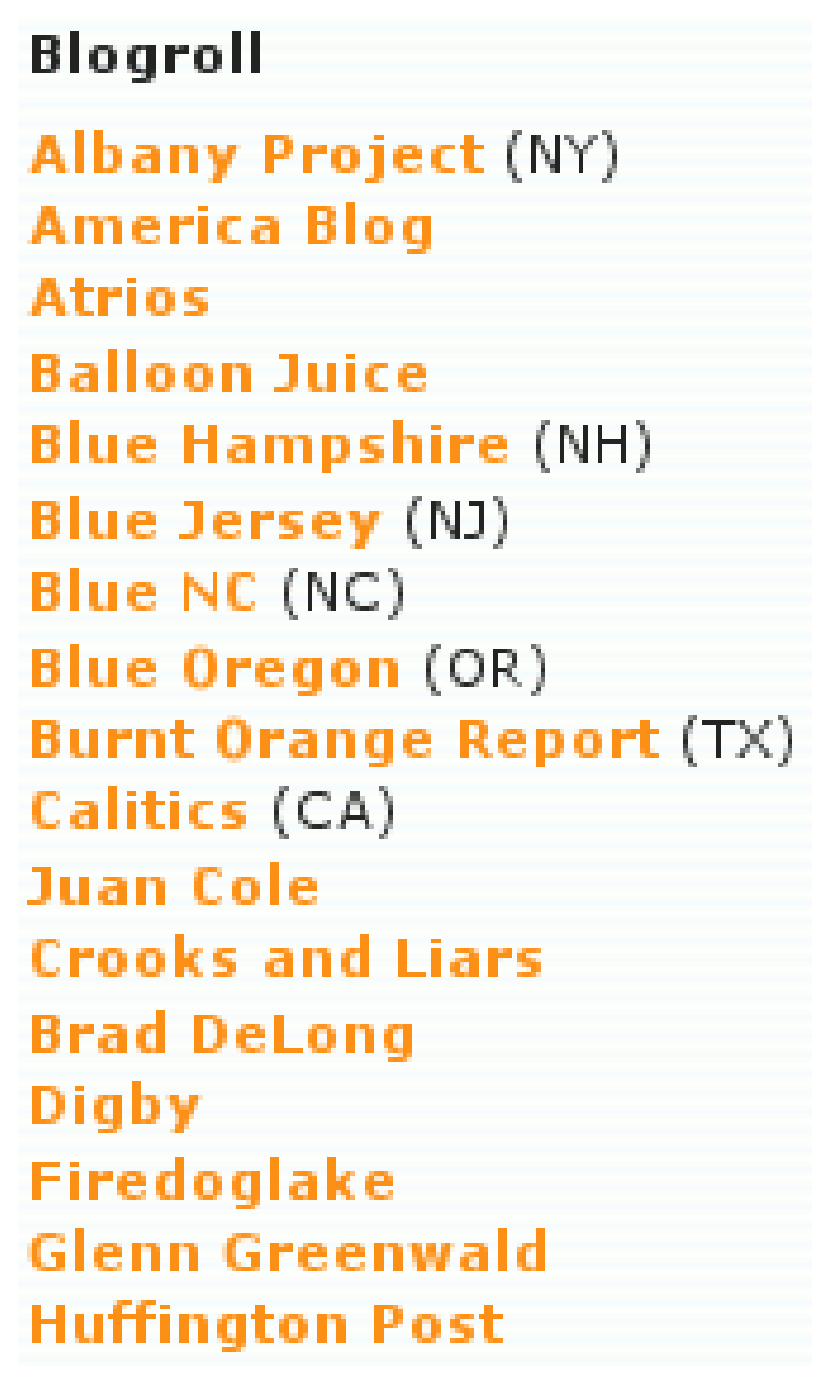
\includegraphics[width=0.9\marginparwidth]{scrsh_dailykos_blogroll}
}

A new phenomena appeared to the mainstream with the introduction of the
\emph{del.icio.us} social bookmarking system. This web page made individual
bookmark collections globally available, making it easy to discover what other
people takes notice of.
%cite, discuss further, lead in to next section.

As \citet[p.~806]{dieberger97} argues the Web's growth, even at it's modest
size of 1997 compared to it's staggering size over 10 years later, have
implications on how easily it is to locate information. By creating pointer
pages, and now socially shared bookmarking services, users are imposing a
structure on the web. By navigating these kinds of interlinked hyperlink
collections it could be that users are getting access to more related and
higher quality information. Sharing a hyperlink, either on you web page or
trough a bookmarking service, requires a conscious effort. One would believe
that people only choose to do so for information they find interesting.

\subsubsection{Item Annotation}
% tagging
% articles with tagging in context of social navigation
% lot of more discussion of tagging and mostly related to organizing
% principles and folksonomy

In addition to being a modern form of pointer pages, social bookmarking
introduced a new way to annotate items. By applying textual key words to
bookmarks--and later other types of content--users were able to browse such
collections in new ways. These key words have been popularized as \emph{tags}
and the act of applying them is called \emph{tagging}. Tagging enables a user
driven odontology and this is often called \emph{folksonomy}.
% cite cite cite cite
Item annotation is often a collaborative process. Some web pages give
suggestions for tags if the item you're annotating have been tagged by others
previously. Users are then more inclined to use some or all of these tags than
to come up with their own. This makes sence if you're annotating a bookmark.
You have your own representation of the bookmark given by the name you gave it
and the tags you choosed to apply. Since a bookmark is distinguished by a
URL others can have other representations of the same resource. For other
content items as photos in a photo sharing site it makes more sence to allow
every user, not only the creator, to apply globaly visible tags.
% cite cite cite cite

\subsubsection{Interaction History}
% in the wild: trailfire, new hoodwink.d like greasemonkey service
% history-rich objects: hill92, hill94

In a classic article \citet{wexelblat99} contrasts the digital world of
computers with our physical world with respect to the formers lack of history.
In our traditional world we exploit such historical information traces
``\ldots to guide our actions, to make choices, and to find things of
importance or interest.'' \citep[p.~270]{wexelblat99} It's argued that this
apparent lack of history in computersized systems must be sorted out such that
future users can take advantage of past users' historical traces left when
they were working on solving problems similar to the current user's. A
possible remedy for this problem on the Web is put forth in the authors'
``Footprints'' system--an navigational aid as an extension to normal web
browsers, visualizing interaction history of past users enabeling current
users to navigate this history.

This interaction history form several navigation trails wich are
``\ldots coherent sequences of nodes followed by an individual.''
\citep[p.~273]{wexelblat99}
The idea of such trails of navigation far preceeded \citeauthor{wexelblat99}
as they were envisioned by \citet{bush45} when he proposed the infamous
theoretical computer-like system named the ``Memex''%
\sidenote[-15\onelineskip]{
  The Memex was not envisioned as a computer system but as an
  electromecanical system consisting of a set of controls hooked up
  to a microfilm reader and camera. It was
  theorized by \citeauthor{bush45} to be a system for handeling
  a persons entire collection of documents, books, and communication.
  It was
  important that a user would be able to access this information with great
  speed and flexibility. An integral part of enabeling such efficient access
  was a user' and content providers' ability to introduce trails between
  information items. \citeauthor{bush45}'s writing about trails
  inspired hypertext \citep[p.~86]{nelson65} wich in turn was the grand idea
  behind the World Wide Web \citep[p.~49]{myers98}.
}.
\citeauthor{bush45} describes a scenario where users are building trails
explicitly, inserts comments if needed, and gives it a name.
\citeauthor{wexelblat99} on the other hand
implemented a system where trails are automatically collected using a set of
heuristics to identify browsing bahaviour representing a coherent navigation
trail.
\citeauthor{bush45} wrote his essay before the invention of computer networks
and he thinks of each Memex as a seperate iseland. Sharing of trails is
possible trough an exportation and following importation process, making it an
explicit action for it's users.
The Footprints system makes the social process of sharing trails implicit and
transparent to it's users--multiplayer is forced.

Controlled user studies by \citeauthor{wexelblat99} did partially falsify
their pre-test hypothesis of Footprint's ability to let users find more
relevant results during a specific browsing task and that this browsing
would be more efficient. The group using the history-enriched system reported
significant lower values of mean page count in their browsing task. No
significantly difference in results returned was found between users of a
plain web browser and users with a browser enhanced with Footprints. They also
found that people experienced in the problem domain of the browsing task were
to a larger degree able to take advantage of interaction history than novices.
\citeauthor{wexelblat99} attributed this to experienced people's ability to
have a clearer mental model of the information one was browsing.

\citet{dieberger00a} modified ``CoWeb''--a collaborative Web space
modelled after Ward Cunningham's famous Wiki--to include interaction history
visualization hoping to make it a more social space, enabeling social
navigation. They visualized other users' access of different pages both by
including a global list of such behaviour and contextual cues about access
next to internal hyperlinks.
It was infered by \citeauthor{dieberger00a} that markers of interaction
history increased the overall activity on the web page during a user study.
They also learned that it's important to both provide both global and
contextual interaction history cues.

% Juggler

\subsubsection{Collaborative Filtering}
% introduce earlier cited goldberg92 article and more recent work. recommender
% systems ties into this

\subsubsection{Recommender Systems}

\subsubsection{Visualization}
% activity, usage, edit/read wear
% footprints users edit/read wear for instance.

\subsubsection{Search}
% social search articles and semantic web/search article
% not that relevant as we're focusing on navigation trough browsing

\subsection{Usefulness}
% dieberger00b:
%   filtering: HEE - find most relevant info
%              RecSys - pick items from a large space
%   quality:   HEE - find quality info (interesting, valid)
%   social affordance: HEE - users aware of each other
%                          - social experience
%                      - space is alive
%                        - not only affect navigation
%                          - stay longer in the space
%                          - relaxed
%                          - try new features

\section{Building on Top of the Web}
% greasemonkey, hoodwink.d, new hoodwink.d service
% browser extensions related, greasemonkey itself a extension, but
% thinking about specialized plugins for enabling interaction on top of other
% web pages.
% mashups kind of related, maybe put inside web2.0 part or separate part
% open apis is the fuel for mashups. possible without by screen scraping, but
% not as convenient and safe (upgrades on the pages we're scraping)
% facebook, open social. apps on top of social network sites. installed base
% of users and relationships already in place.


    \chapter{Methodology}
\label{chapter:methodology}

This chapter will include information in how data was collected. So far this
includes content inventory/analysis.

\section{Content Analysis}

The term \term{content analysis} is traditionally used to signify a
qualitative research method used in the social sciences.
\prequote[\p{18}]{krippendorff03}{defines it as}{%
  a research technique for making replicable and valid
  inferences from texts (or other meaningful matter) to the contexts of their
  use}
Even though such an analysis of the contents, meanings, or effects of
communication messages also have been utilized on the Web \citep{weare00}
it does not seem very well suited for understanding navigational mechanisms.

We turn to content analysis as the more pragmatic practice conducted within
the field of \term{information architecture}%
\sidenote{
  Information architecture can be explained as
  \begin{inparaenum}[(i)]
    \item the structural design of shared information environments,
    \item the combination of organization, labeling, search, and navigation
      systems within web sites and intranets,
    \item the art and science of shaping information products and experiences
      to support usability and findability, and
    \item an emerging discipline and community of practice focused on bringing
      principles of design and architecture to the digital landscape
      \citep[\p{4}]{morville06}.
  \end{inparaenum}
} hoping that it will help us get an better understanding of navigational
structures.
Content analysis is deployed as a technique by information architects for
helping them generate a sound and well structured web site architecture.
It's seen as a bottom-up process and
in its essence a content analysis should identify the various
relationships (or lack of correlation) between a web site's content items.
It consists of two phases:
\begin{inparaenum}[(i)]
  \item a collection of a representative sample of data and
  \item an analysis of this collected data
\end{inparaenum}
\citep[\pp{241}{243}]{morville06}.

Information architects are concerned with
the system's content and
\postquote[\p{94}]{batley07}{%
  need to move below the surface of the system
  interface to examine the system information itself}
We on the other hand are actually concerned with the system interface and
specifically its navigational structures. This creates a striking
contradiction as we're not interested in content unless it can help or
guide users during their navigation. We therefore have to adapt
both our inventory and analysis process accordingly.

\subsection{Inventory}

A \term{content inventory} is a technique for collecting data from web sites
in a structured manner. It's strength as a technique lies in its ability of
truly informing about a web site's content \citep{wodtke02}. The process of
actually conducting a content inventory can be equally rewarding as the
resulting documents \citep{veen02}.

\subsubsection{Sampling}
\label{section:methodology.content.analysis.sampling}

Content inventories are often tedious and time consuming to perform.
\citet[\p{267}]{wodtke02} argues that every single bit of content needs to be
determined while \citet[\p{241}]{morville06} believes a representative sample
is sufficient.

The web sites that are interesting to look at in our research are vast and
loaded with enormous amounts of user generated content. An all-inclusive
approach to content gathering would simply be impossible in such situations.
As a remedy to this we've decided to ignore certain parts of web sites in our
content inventories since the scope of our research is limited to navigational
constructs and only those which have a social nature.

Our experience is that social navigation and more static navigation are
intermixed all over web sites. Often one have to use non-social forms of
navigation before social navigational options appear. Thus we could not simply
ignore navigational aims which were non-social in our content inventory phase.
We did however eliminate the following parts of web sites under investigation:

\begin{enum}
  \iterm{Administrative sections} where users can change their profiles or set
    their preferences.
  \iterm{Help pages} where \abbr{FAQ}s, guides, and instructions are presented
    in a static manner.
  \iterm{Legal information} including terms of service, privacy policies, and
    copyright notices.
  \iterm{Content generation} facilities like uploading, categorizing, and
    editing photos, commenting, posting items, and so on%
    \sidenote[-10]{
      While there is no question about the usefulness of such content for
      providing social navigation possibilities we've found few examples where
      social navigation is used in the content generation phases itself.
      There is however a few exceptions and these will be discussed when
      appropriate. % collaborative tagging for instance
    }.
  % to be extended when more sites are investigated
  \iterm{Advertisements} from third party advertisers.
\end{enum}

In addition to eliminating certain form of web pages we synthesized abstract
page representations by introducing variables. Take for example a typical
social network site. There are from thousands to several millions of
profile pages. In context of what navigational options these pages present to
us they are all essential similar. So we could introduce a variable called
\var{user-name}%
\sidenote[-5]{
  The variable notation with a dollar (\$) prefix is inspired from
  variable usage in \abbr{UNIX} shell scripting \citep[\p{88}]{kernighan84}.
}
and thereby describe all potential profile pages as:
\val{Profile of \var{user-name}},

We would however have to make sure that the one page we used in our inventory
to represent the abstract notion of a profile page was representative. To
exemplify, say that a profile page included a stream of the 10 most recent
actions your friends had conducted. If the user of our collected profile page
had zero friends we would lack the navigational opportunities such a stream
could give us in our inventory. Therefore we used only pages which provided
all possible forms of navigation as basis for abstraction.

\subsubsection{Approach}

We started out on the first page that was given us when entering the web site
under investigation. From there we stepped trough each page of the web site
by following all navigational hyperlinks provided on individual pages.
We did not however frequent a web site in its entirety, but bearing in mind
our sampling constraints and abstractions we frequented the site to full
coverage. We stopped browsing a particular page if it%
\sidenote{
  Either the exact same page or a page deemed to be the same by our
  variable driven abstraction method.
}
had been previously been inventoried. During the course of this browsing
each page was noted down in a table with the following characteristics:

\begin{enum}
  \iterm{Identifier} of numerical and hierarchical form where page with id
    4.3.1 is the first child of a page with id 4.3, representing its place in
    the navigation structure. The first page was given an id of \val{0},
    its first descendant an id of \val{1} and so on.
  \iterm{Page title} as a description of what the page contains. Some of the
    web site's we surveyed had a slight ambiguity of title usage. In these
    cases we decided to collect the most representative sample%
    \sidenote{
      A choice between the \code{<title>} element in the \code{<head>}
      of the \abbr{HTML} document and the \code{<h1>} top level heading
      in-line the \code{<body>} portion of the document was made.
    }.
    If this resulted in unsatisfactory results we created a new title using
    the best of our abilities to make it as clear and descriptive as possible.
  \iterm{Link name} is either the textual name or a description of the
    contents (i.e. a graphical representation) of the hyperlink that was
    utilized to navigate to this very page.
  \iterm{Link location} as a description of the spatial position
    (for example: global navigation, content area, right sidebar) of the
    hyperlink used to navigate to this page.
  \iterm{Page \abbr{URL}} as an identifier for the page we visited.
\end{enum}

The result was a table representing a web site's various pages and the
navigational relationships amongst them.

While we took note of the \abbr{URL} of each page we've decided not to display
this information. We're not convinced of its usefulness in light of
navigation and therefore for brevity sake omitted them. We did however use
them in our inventory process as a way to identify previously collected pages.
We were able to clearly distinguish between different pages
by introducing variables into the \abbr{URL}s as well.

In a traditional content inventory other characteristics
is usually collected. For an example see \citet[\p{269}]{wodtke02}.
As we described earlier we're only concerned with the navigational parts of
web pages. We opted to only record what we found to be useful for this
purpose. This lead to a situation where we were collecting more information
about site structure than the attributes of a site's content\dash{}as an
information architect usually would do.

\subsection{Analysis}

An analysis of the collected content follows after an inventory phase is
completed. Typically information architects use content analysis for
making decisions on what and how to improve an existing web site's content
architecture. With such an aim they look for patterns and relationships when
analyzing their content inventory. These patterns and relationships will then
suggest groupings and connections amongst separate content items
\cite[\p{243}]{morville06}. For an example of further issues that information
architects tends to focus on see \citet{leise07} and his set of 11 heuristics%
\sidenote{
  The heuristics, shortly summarized, are:
  collocation,
  differentiation,
  completeness,
  information scent,
  bounded horizons,
  accessibility,
  multiple access paths,
  appropriate structure,
  consistency,
  audience-relevance, and
  currency.
}
for content analysis.

\subsubsection{Approach}
Since our focus were dissimilar compared to that of most information
architects' we've had to tailor the analysis process to best help us discover
and understand patterns of social navigation in web sites. Analyzing content
inventories for such means is as far as we know not conducted before. We were
therefore exploring unknown waters and had to adapt our method as we
went about with our analysis.

We started with our impressions from the content inventory%
\sidenote{
  As stated earlier the process of conducting a content inventory is not only
  beneficial just because of the resulting documentation one creates of a web
  site. People conducting content inventories tends to get deeply informed
  about a web sites content and structure after having exhaustively recorded
  large parts of it. 
}
and based our discussion on the findings we regard most conspicuous in
relation to social navigation. During the resulting discussion we tried to
reference the pages recorded in our content inventory by their identifiers.

\section{User Testing}
\label{section:methodology.user.testing}

Testing of real world users over time with an experiment and control group.

    \chapter{Analysis of Social Navigation in Modern Web Sites}
\label{chapter:analysis}

This chapter will include a survey and analysis of the data we've collected
which can be found in it's whole in
Appendix~\ref{appendix:content.inventory}
(p.~\pageref{appendix:content.inventory}).

\section{Flickr}

\sidefigure{Flickr Photo Meta-data}{%
  Photo Meta-data,
  retrieved October 28, 2007, from
  \url{http://flickr.com/photos/benbengraves/187609810/}.
}{%
  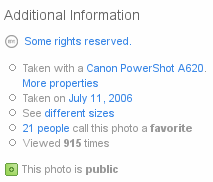
\includegraphics[width=\marginparwidth]{scrsh_flickr_photo_detail_metadata}
  \label{figure:scrsh.flickr.photo.detail.metadata}
}

Flickr is a photo sharing site which are known to be on the cutting edge when
it comes to enabling new and innovating features in it's domain. Flickr has a
quite peculiar history as it started out as a massively multi player online
game. An environment for photo sharing within the game was added in 2004 which
quickly became more popular than the game itself. The focus of the company was
shifted and their new photo sharing community was bought by Yahoo! Inc. in
March 2005 \citep[p.~257]{livingston07}.

This subsequent
analysis of Flickr will be carried out as a registered user. One has to be
registered for interacting with the site in such a way that one leaves
persistent traces. The site has a open nature enabling anonymous access
to the majority of content.

\subsection{Thumbnails}

Already on the welcome page (Figure~\ref{figure:scrsh.flickr.welcome},
p.~\pageref{figure:scrsh.flickr.welcome})
we're finding navigation links that are social of
nature. Four thumbnails functions as sample of the most recently uploaded
photos by other members of the community. One can either navigate straight to
a detailed page for each particular photo by clicking on the respective
thumbnail (Id 6, p.~\pageref{table:flickr.content.inventory.6})
or the profile of the uploader by clicking on their user
name (Id 7, p.~\pageref{table:flickr.content.inventory.7}). Such thumbnails
with minimal meta data (the uploader) are prevalent all over Flickr. Of the
120 pages we collected in our content inventory 26 of them contained
thumbnails. Most of these thumbnails
are giving users incentives to navigate using social means%
\sidefill
\sidenote{Apart from the few pages that only show a
          stream of your own thumbnails--when you're browsing your
          own photos by various methods.}.
Which photos these thumbnails portray is dynamic. That is to say that other
users' actions--uploading a photo, tagging a photo, taking a photo with a
specific camera, collecting photos into sets, and adding photos to a certain
group--all determine the navigational choices you as a user is
presented with.

\subsection{Meta-data}

We arrive on a photo detail page as in
Figure~\ref{figure:scrsh.flickr.photo.detail}
(p.~\pageref{figure:scrsh.flickr.photo.detail})
if we utilize one of these thumbnails for navigation. In addition to comments
on the photo we find meta-data as in 
Figure~\ref{figure:scrsh.flickr.photo.detail.metadata}
(p.~\pageref{figure:scrsh.flickr.photo.detail.metadata}).
Meta-data include the date the photo was taken, the manufacturer and the model
of the camera that was used which are all so called Exif%
\sidenote{Exchangeable Image File: a specification for image file format used
in digital cameras.}
data. Flickr utilize this data by enabling navigation based both on the
dates a picture was taken and by camera make and model. Say you're trying to
find a picture from your home town on a particularly beautiful summer day. By
using date of picture taking based navigation coupled with tags or
geographical data (which both will be discussed shortly) you're probably
increasing you chances of finding what you want. Camera make information could
be useful when looking at the quality of pictures taken with certain cameras
before purchasing one yourself.

\begin{figure}[b]
  \captionstyle{\raggedright}
  \begin{whole}
    \begin{minipage}[t]{0.475\wholewidth}
      
\includegraphics[width=\textwidth]{scrsh_flickr_welcome}
      \caption[Flickr Welcome Page]{%
         The Welcome Page,
         retrieved October 16, 2007, from \url{http://flickr.com}.}
      \label{figure:scrsh.flickr.welcome}
    \end{minipage}
    \hfill
    \begin{minipage}[t]{0.475\wholewidth}
      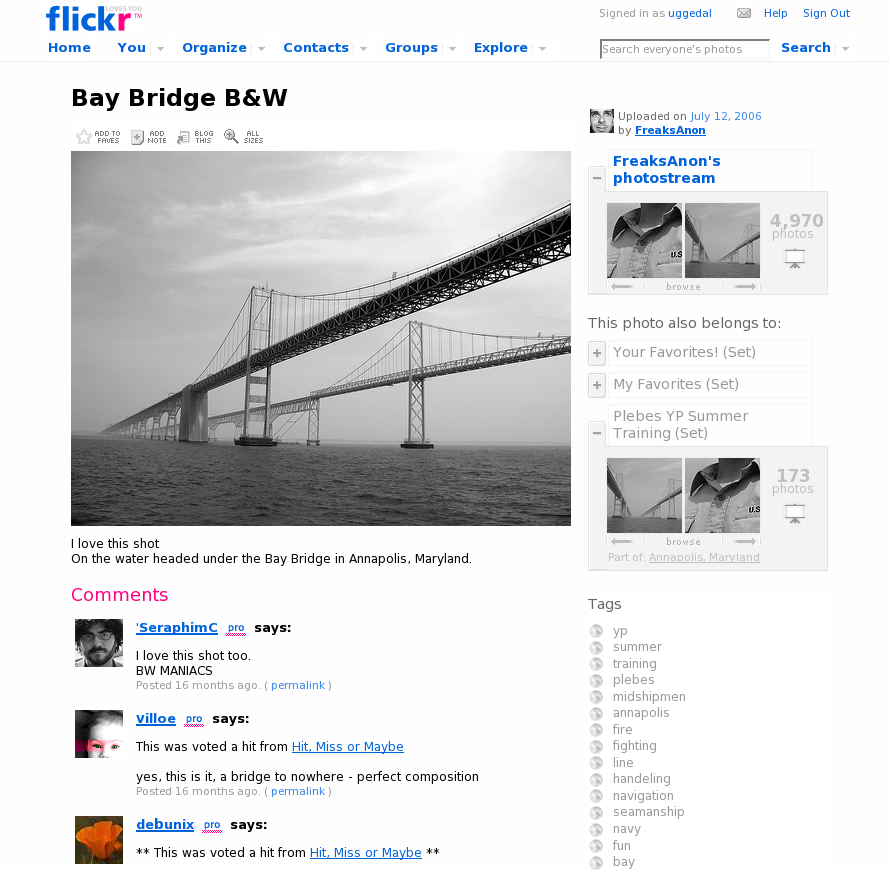
\includegraphics[width=\textwidth]{scrsh_flickr_photo_detail}
      \caption[Flickr Photo Detail Page]{%
         A Photo Detail Page,
         retrieved October 26, 2007, from
         \url{http://flickr.com/photos/benbengraves/187609810}.}
      \label{figure:scrsh.flickr.photo.detail}
    \end{minipage}
  \end{whole}
  \normalcaption
\end{figure}

\subsection{Folksonomy}
Of most importance
for Flickr, and indeed what makes Flickr a folksonomy, is it's tagging
abilities. Caterina Fake, co-founder of Flickr, explains it's importance:
``Tagging really revolutionized the way the product behaved.''
\citep[p.~261]{livingston07}
All
registered user can label anyone's photos by applying such short descriptive
tags. This collaborative process lay the ground work for other user's ability
to easily browse photos by topic.
Figure~\ref{figure:scrsh.flickr.tagcloud}
(p.~\pageref{figure:scrsh.flickr.tagcloud}) exemplifies how the user generated
data trough tagging can be used as a navigational aid. A so called \emph{tag
cloud} is used to visualize the popularity (and thereby importance) of the
individual tags. The larger the tag title, the more frequent the tag has been
applied to photographs.

Tag clustering was released in the fall of 2005 \citep{butterfield05} as a way
to easier see the relationships between separate tags. For any given tag a
cluster of three related tags is generated and displayed to users when they
are browsing as seen in
Figure~\ref{figure:scrsh.flickr.photo.detail}
(p.~\pageref{figure:scrsh.flickr.photo.detail}). Flickr algorithmically
generates these listings based on what tags users tend to use together for
labeling a photo.

Tagging is a very flexible approach only hindered by users' imagination. In the
early days of Flickr there was no support for geographical data. Users soon
found a remedy for this by tagging photos with longitude and latitude. By
using the same technology we're using in our prototype application
(Greasemonkey) they were able to integrate Google Maps%
\sidefill
\sidenote{
  Available at \url{http://maps.google.com}
} in Flickr, enabling user's to place their photos on a map and automatically
generate geographical coordinate tags%
\sidenote{
  More info about the early days of \emph{geotagging} can be found on the
  remains of the Flickr Geotagging group, available at
  \url{flickr.com/groups/geotagging/}.
}.

\subsection{Geographical data}

In late August 2006 Flickr introduced geotagging abilities
\citep{butterfield06} by integrating mapping aspects from Yahoo! Maps%
\sidenote{
  Available at \url{http://maps.yahoo.com}.
}
Users could now place their photos on a
map to signify where they were captured.
% Finish description.
% Take screen shot.
% Write about the new places feature.
% Write and cite when proper geo data was incorporated.

\subsection{Interestingness}
% Cite collaborative filtering. Introduced in same blog post as clustering.

\begin{figure}[b]
  \begin{whole}
    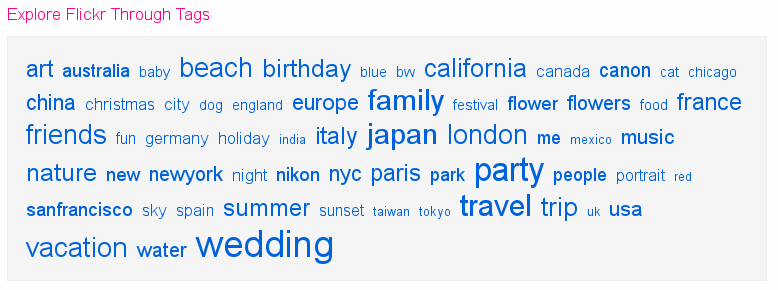
\includegraphics[width=\wholewidth]{scrsh_flickr_tagcloud}
    \caption[Flickr Tag Cloud]{%
       Tag Cloud,
       retrieved November 1, 2007, from \url{http://flickr.com/explore}.}
    \label{figure:scrsh.flickr.tagcloud}
  \end{whole}
\end{figure}

\begin{figure}[b]
  \begin{whole}
    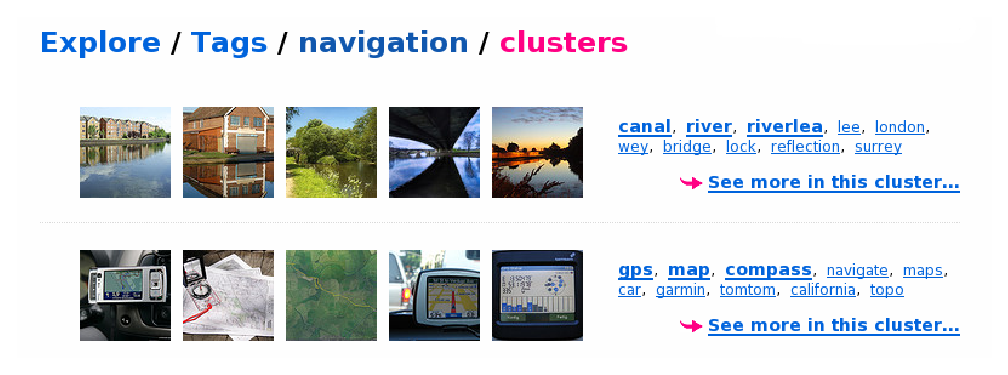
\includegraphics[width=\wholewidth]{scrsh_flickr_tagcluster}
    \caption[Flickr Tag Cluster]{%
       Tag Cluster,
       retrieved November 19, 2007, from
       \url{http://flickr.com/photos/tags/navigation/clusters/}.}
    \label{figure:scrsh.flickr.tagcluster}
  \end{whole}
\end{figure}

    \chapter{Implementation}
\label{chapter:implementation}

As we've seen in 
\sectionref{building.on.top.of.the.web}
it's possible to build applications on top of existing web sites by creating
transparent prototype implementations. This chapter starts with an account of
what kind of navigation system we wanted to build, goes on to describe why we
decided on such navigational designs, and concludes with an explanation of the
deeper technical decisions we had to make. The following chapter,
\chapterref{selection.of.third.party.software},
describes what kind of third party software we used for realizing the
implementation details we describe in this chapter.

\section{Design}

When we're talking about design we mean how the application we're making is
presented to users. For discussion of how the software is designed
or architected internally, take a look at
\sectionref{implementation.architecture}.

Our philosophy when creating a navigational design have been
similar to that practiced by
\begin{fullquotation}[\chap{3}]{exupery67}{in aviation design}
  \noindent
  And now, having spoken of the men born of the pilot's craft, I shall say
  something about the tool with which they work, the airplane Have you
  ever looked at a modern airplane? Have you followed from year to year
  the evolution of its lines? Have you ever thought, not only about the
  airplane, but about whatever man builds, that all of man's industrial
  efforts, all his computations and calculations, all the nights spent
  over working draughts and blueprints, invariably culminate in the
  production of a thing whose sole and guiding principle is the ultimate
  principle of simplicity?

  It is as if there were a natural law which ordained that to achieve this
  end, to refine the curve of a piece of furniture, or a ship's keel, or
  the fuselage of an airplane, until gradually it partakes of the
  elementary purity of the curve of a human breast or shoulder, there must
  be the experimentation of several generations of craftsmen. In anything
  at all, perfection is finally attained not when there is no longer
  anything to add, but when there is no longer anything to take away,
  when a body has been stripped down to its nakedness.
\end{fullquotation}

This philosophy is closely related to minimalism, a movement where the
infamous architect Mies van der Rohe popularized the concept of
\q{less is more}\dash{}achieving the maximum effect with the minimum of
means \citep{whitman69}.
That is why we feel the application we're creating should provide users
with only the necessary information for affording navigational behavior.

\citet{schwartz04} wrote a book called
\work{The Paradox of Choice: Why More Is Less} in which he explains that
we in our modern society have an overabundance of choice. All these choices
can produce psychological distress. As \citeauthor{schwartz04} explains this
problem can be resolved by limiting the amount of choices we are presented
with.

Our design could potentially introduce even more choices. We're
introducing more information, and more navigational choices, into the
\urort{} web site. A possible solution could be to remove some of the
choices presented to the user if we felt the choices we're providing in
regards to navigation were of higher importance than those provided by
default. We decided against this since we want to test our navigational
design in opposition to the navigational designs already provided. By
eliminating some of the default navigation we would not be sure
if potentially more satisfied users was the result of our removal of
choices or the new choices we provided.

\subsection{Activity Feed for \urort{}}

According to \prequote[\p{193}]{dubinko07}{}{%
  There is enormous and growing interest in the consumption of up-to-the-
  moment streams of newly published content of various forms: news articles,
  posts on blogs or bulletin boards, and multimedia data such as images,
  songs, or movie clips}

In the \urort{} web page there is currently not an easy way to discover what
is new for the areas that you personally care about. The main page
as seen in \figureref{scrsh.urort.main.page}
displays the latest editorial articles and in some sense they represent
new content. At the right margin there are also lists of both editorial song
selections and the most popular by listenings and downloads. Whether you're
logged in to the web page by a registered user handle or browsing the page
anonymously you're presented with the same information. Navigating onto your
personal profile page yields the same results: no good pointers to fresh
content.

\begin{figure}
  \begin{whole}
    \centering
    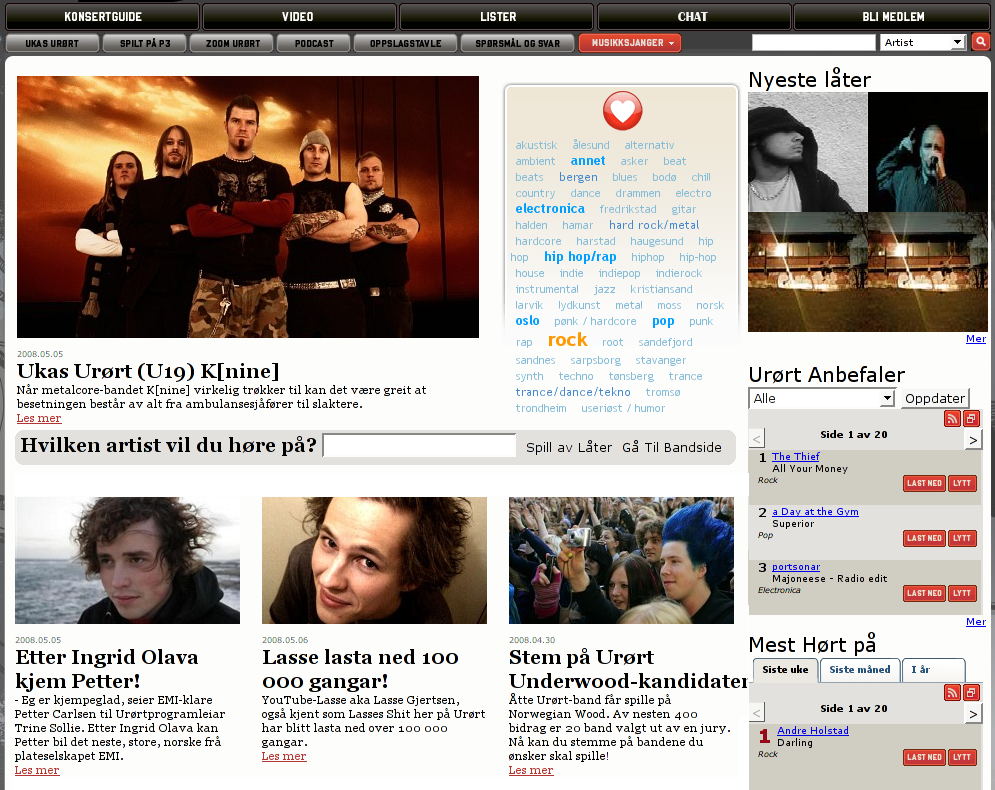
\includegraphics[width=0.9\wholewidth]{scrsh_urort_main_page}
    \caption[\urort{} Main Page]{
      The main page of \urort{},
      retrieved May 8, 2008, from
      \url{http://www11.nrk.no/urort/default.aspx}.
    }
    \label{figure:scrsh.urort.main.page}
  \end{whole}
\end{figure}

When we conducted our study of the Facebook social network site we came
intrigued by how easy it was to keep updated on the latest developments for
our friends by using its news feed as described in
\sectionref{analysis.facebook.news.feed}. 
Such feeds of activity seem to have become popular also outside Facebook.
\project{Socialthing!} and \project{FriendFeed} are two services that
aggregates such feeds from several sources and provides an unified feed. Their
distinguishing factor is that Socialthing! fetches activities for your
existing friends on services as Facebook and Flickr. FriendFeed on the other
hand only collect activities from the people you decide to follow on
FriendFeed itself. In addition FriendFeed can display your personal feed
as an aggregation of all supported services you're using. Both activity feed
aggregators are shown in \figureref{scrsh.friendfeed.me} and
\figureref{scrsh.socialthing}.

\begin{figure}
  \begin{whole}
    \centering
    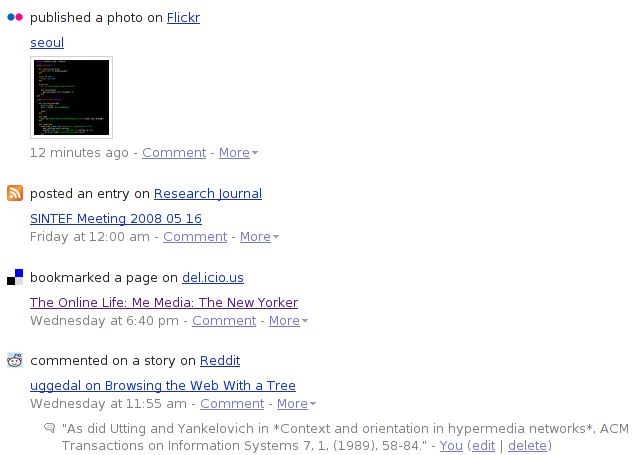
\includegraphics[width=0.9\wholewidth]{scrsh_friendfeed_me}
    \caption[FriendFeed Activity Feed]{
      Activity feed for the author on FriendFeed,
      retrieved May 18, 2008, from
      \url{http://friendfeed.com/uggedal}.
    }
    \label{figure:scrsh.friendfeed.me}
  \end{whole}
\end{figure}

\begin{figure}
  \begin{whole}
    \centering
    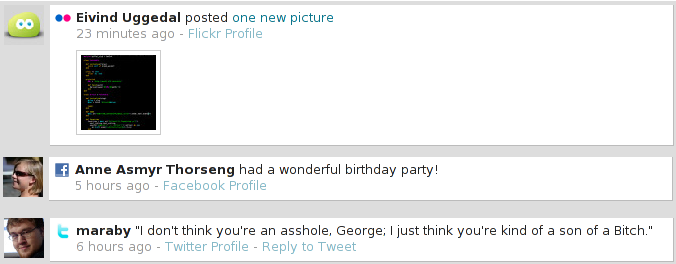
\includegraphics[width=0.9\wholewidth]{scrsh_socialthing}
    \caption[Socialthing! Activity Feed]{
      Activity feed for the author and his friends on Socialthing!,
      retrieved May 18, 2008, from
      \url{https://socialthing.com/}.
    }
    \label{figure:scrsh.socialthing}
  \end{whole}
\end{figure}

\subsubsection{Relevant Activities}

The approach seen at Facebook for letting users know what's fresh and relevant
for yourself trough an activity feed seemed a good fit for \urort{}. But
\urort{} does not have the concept of friends as seen in social network sites.
\urort{} exists for people to freely share their music and let others find
music they like\dash{}and not on making new friends or keeping in touch with
old friends. How do we then find recent activities which potentially could be
interesting for our users when we don't have any frinds to consult?

We tried to answer this question by using a feature on \urort{} that allows
any user to \emph{favorize} an artist. If a user conducts such an action he or
she becomes a \emph{fan} of that artist. We don't know why people signify
artists as their favorites on \urort{}, but the main reason may be that
they simply like the music the artist is publishing.
Another reason could be that people know the artist personally and therefore
add them as a favorite\dash{}not dependent on whether they like their music or
not.

But regardless of the motives for adding an artist as a favorite it requires
a concious effort from the user. We're therefore led to believe that the list
of artists a user have favorized are more important than other artists on
\urort{}. Our design is therefore based on the activities of a person's
favorite artists. Initially we toyed with making a friend like concept on
\urort{} by saying that people which share one or more favorite artists with
you are in some way related to yourself. We had to trow away this idea because
of technical problems with getting such a solution to scale.

\subsubsection{Activity Types}

There were many activities taking place associated with an artist
which we could potentially use in our activity feed. We decided to select
those which had information about when the activity occured and was
technically easy%
\sidenote{
  Easy as in only requireing access to the \urort{} web pages.
}
to retrieve. Those that matched our criteria was:

\begin{items}
  \iterm{Songs} beeing published by the artist.
  \iterm{Song reviews} beeing written by users.
  \iterm{Concerts} beeing performed by the artist.
  \iterm{Blog posts} beeing written by the artist.
\end{items}

As you can see three of these activities are conducted by the artist himself
while reviews are conducted by other users.

\subsubsection{Activity Filtering}

There is quite bit of activity information based on our four categories for
a typical artist. When a user have several artists as favorites the ammount of
activity information gets large. We therefore had to filter out some
activities and only showing what we thought would be most relevant.

Firstly we're only concerned with historical information in our activity list.
Future concert events are therefore filtered out. Secondly we're showing the
most recent activities believing that fresh content is more important than
aged content. As activities are sorted chronologically in our feed we simply
cut off all activities after a preset number of the most recent activities are
displayed. The version of our prototype which was tested by real world users
showed only the ten most recent activities.

Facebook is not showing the complete picture of friend activity in their news
feed as it's believed that up to 80\% of all recent activities are filtered
out \citep{mccrea08}.
Facebooks approach to only showing a selection of recent activity is
probably driven by technical scalability problems, and not a desire to only
present a selection of recent activity of friends. In our activity feed we
give users a complete picture of all our types of activities within our
cut-off point.
The complete design of our activity feed for \urort{} can be seen in
\figureref{scrsh.urort.activity.feed}.

\begin{figure}
  \centering
  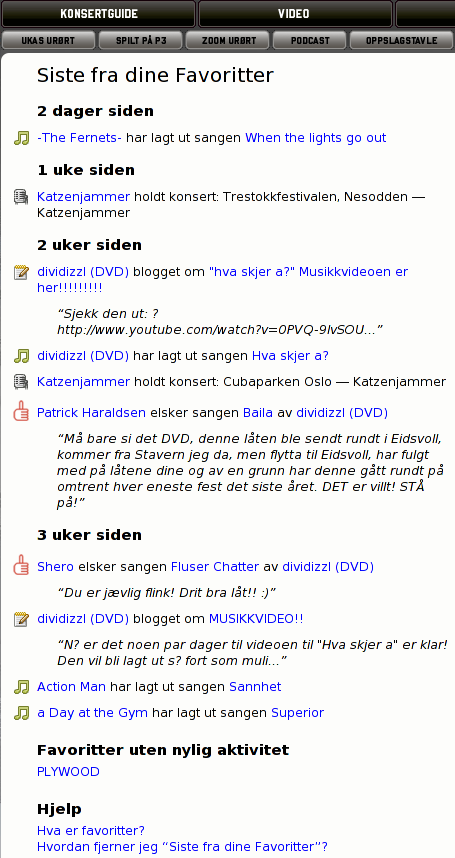
\includegraphics[width=0.9\textwidth]{scrsh_urort_activity_feed}
  \caption[\urort{} Activity Feed]{
    Activity feed for experiment users on \urort{},
    retrieved Jun 2, 2008, from
    \url{http://www11.nrk.no/urort/default.aspx}.
  }
  \label{figure:scrsh.urort.activity.feed}
\end{figure}

\subsection{Favorite List}
\label{section:implementation.design.favorite.list}

As described in
\sectionref{methodology.user.testing}
we decided to used a control group in our user testing. The navigational
design we presented them with did not include an activity feed. In stead they
simply were presented with a list of their favorites so that they manually had
to keep up with what recent activity their favorite artists were conducting.
The design of the control group implementation can be seen in
\figureref{scrsh.urort.favorite.list}.

To give both our control and experiment group the same navigation
possibilities\dash{}excluding the activity feed\dash{}we decided to show a
list of the favorites without recent activity for our experiment group. If all
their favorites had activities present in the feed no such list was displayed.
\figureref{scrsh.urort.activity.feed} shows the listing of one such artist
without recent activity.

\begin{figure}
  \centering
  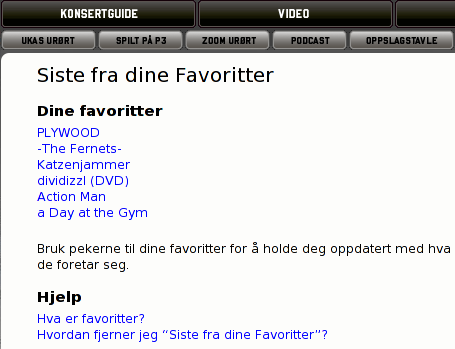
\includegraphics[width=0.9\textwidth]{scrsh_urort_favorite_list}
  \caption[\urort{} Favorite List]{
    Favorite list for control users on \urort{},
    retrieved Jun 2, 2008, from
    \url{http://www11.nrk.no/urort/default.aspx}.
  }
  \label{figure:scrsh.urort.favorite.list}
\end{figure}

\section{Installation}

We did our best to make the installation process of our prototype easy
for end-users. This is important for getting as many people using our
prototype as possible.
Descriptive, stepwise instructions with screenshots for the installation of
the components of our client software was provided.

\section{Process}

\subsection{Prototyping}

A \term{prototype} is an early version of an application that are used for
finding out more about the problem at hand and its possible solutions
\citep[\p{409}]{sommerville06}.
The software developed for our research on social navigation fits these
characteristics. It's not supposed to be used after its behavior is
evaluated. For that it's to inefficient and relies on specific web browser
environments and extensions. This does not mean that the prototype can't have
impact on how \urort{} evolves in the future. If our evaluation favors our
design decisions the developers of \urort{} might take advantage of such
potential improvements in their web site design.

\citet[\pp{409}{410}]{sommerville06} explains that a prototype can be used for
\begin{inparaenum}[(i)]
  \item gathering more sound requirements from users during a
    requirements phase,
  \item evaluating the feasibility of a proposed design during a
    design phase, and
  \item testing the final system by verifying it against the prototype.
\end{inparaenum}
We're following his second example of prototype usage by making a prototype
for what we believe to be a sound social navigation design. This is then
evaluated. If time permitted (sadly one has limited time and resources
available during master thesis research) the results of such an evaluation
could be input in a new design process and a new prototype system.

As \citet[\p{114}]{mcconnell04} explains prototyping can mean different things
based on context. Often it's used to explain systems where one writes the
least amount of code to get a solution and throw it all away when the design
question is answered. This is not our intention. We'll try to make the system
fully operational and make the code we author comprehensible and
valid. More precisely we're creating a \term{high-fidelity} prototype
\cite[\p{78}]{rudd96} with a robust architecture.

The reason to create a robust application is twofold. Firstly we're developing
the prototype as part of our master thesis and it's meant to show how
proficient we are in both programming and designing applications. We
imagine delivering a barely working and poorly constructed software package
would not be beneficial for our examination results.
Secondly the application could potentially see some stress under user testing
depending how large the test population is. Having a crashing or
non-functioning application during such testing could prove to be costly.

We're therefore creating a prototype to demonstrate our ability (or inability)
to develop software. This is not our sole reason, and probably not the most
important. As \citet[\p{292}]{mayhew90} describes prototyping is not
successful if one have not learned something during the process about what one
set out to investigate at the outset. We want to investigate navigational
designs an the prototype is with such a focus nearly a means to an end.

\subsection{Testing}
\label{section:implementation.process.testing}

One can verify that the application one are building functions as it's
supposed to do as code is added and changed by using automated tests.
We have personally experienced benefits with using automated testing on
earlier projects.
\term{Test-driven development} is a development technique
where one writes an automated test for a non-existent feature or
improvement before one actually implement the feature itself\dash{}development
is literally driven by tests. So the focus is not primarily on the test, but
to better design software trough a test-first approach.
\citet{janzen08} conducted studies
on both developers in companies and university students for finding out
whether a test-driven approach improved the quality of software design.
Groups which wrote a test before the accompanying code were measured
against groups which wrote their test after implementing the solution.
They found that code size decreased when a test-first approach was
used\dash{}both classes and methods were smaller and simpler. In addition
test-first developers had better coverage of the implementation code in
their tests \citep[\p{81}]{janzen08}. This could indicate that it's
easier to choose not to implement tests after you have a piece
of working code. The discipline that test-driven development dictates
makes it impossible not to write tests.

\term{Behavior-driven development} is a response to the test-driven
development approach introduced by \citeauthor{north06} for shifting the focus
from writing tests to writing specifications of behavior
\citep{north06}. By writing specifications one is able to
more clearly describe the intent of an application than when one
are writing traditional tests.

We are convinced of the benefits of behavior-driven development based on
earlier development projects and are therefore developing our
prototype application with such a development process. Having specifications
that can be automatically run to check how our application conforms to our
expectations is very valuable. This is especially so when we're working
with \urort{} as an external data source since we don't have control over
the stability of its structure.

\section{Architecture}
\label{section:implementation.architecture}

Our implementation basically needs to do two things:

\begin{enum}
  \item Collect existing data from various places on the \urort{} web site.
  \item Display this data in existing web pages on the \urort{} web site in
    a way that we hope will enhance navigation.
\end{enum}

\subsection{Extending an Established Web Site}

As we've described earlier in this chapter we're creating a prototype
application. Inspired by solutions in the Hoodwink.d community we set
out to implement our system on top of already established web pages as
described in \sectionref{building.on.top.of.the.web}.

\citet{laird07} makes a case for using the means of such a browser
extension\dash{}Greasemonkey\dash{}and custom scripts for
realizing projects that without such technology would
never have come to existence. As he describe there is a sweet spot where such
an approach really shines. He therefore created a framework for determining
if a given project embodies the factors that would make this kind of an
implementation a particularly suitable solution. What follows is a recitation
of his selection factors and how our project adheres to these.

\subsubsection{Do you have access to the source code of the web application?}

When the source code of the target web site is available it would probably
be easier to just change that. The case is made for using Greasemonkey when
the source code is not available. Since we don't have access to the internals
of \urort{} we see this factor as favorable for Greasemonkey in our project.

\subsubsection{If the application is under your control and source code is
  available, is updating the application a risky endeavor?}

This factor does not apply to our implementation since we obviously did not
create \urort{} ourselves. Had we done that we could have used
Greasemonkey for adding new features without putting the existing web
site in danger as it would be externalized from the original implementation.

\subsubsection{How critical is the feature to be added?}

If the web site is not functional or complete without the new feature
it is advisable to defer from using Greasemonkey. The reason is the
difficulty of ensuring that all users have the extension installed
and the newest version of the custom script. Since we will be able
to ensure that our test users have the right extension and scripts
installed this is of no concern to us. In addition \urort{} is
functioning fine without our feature enhancement which makes
Greasemonkey a sound technical solution for our means regarding this factor.


\subsubsection{Is Firefox available for the potential users, and does it
  work with the target application?}

The Firefox web browser should be available to install on most platforms
and we can report that it works fine on the target web site.

\subsubsection{To what degree are the target users computer literate?}

Installing a web browser, an extension for it, and finally a custom script
can be a bit complicated for certain users. We have to expect the
test users to be a selection of our general population and some could
therefore have trouble with achieving such a setup. On this aspect
a solution that alters the original application would work better
since users are not required to change their computing environment.
We hope to partly solve this problem with providing clear instructions
for how users can configure their environments to support custom
Greasemonkey scripts.

\subsubsection{What size is the user population that needs the new feature?}

This factor is based around the fact that server applications can be more
easily updated since they seldom require intervention by the user. It's
much harder to ensure that client applications like Greasemonkey are
kept up-to-date by its users. It's argued that such an approach works
better for smaller populations and one should therefore keep users
of custom Greasemonkey scripts to a minimum.

Since we're not foreseeing the use of our implementation outside user
testing the application does not have to be kept up to date. In addition
we're anticipating a fairly limited user base due to our test setting.
Greasemonkey should therefore not put any hindrance in place for
our implementation in relation to this factor.

\subsubsection{Is the application exposed to the public internet?}

This factor relates to the previous about keeping the user base limited.
In addition to limiting the size of your user population it's also
important to know them\dash{}know who your users are\dash{}so that
one more easily can support them if need be. Since our application
only will be available to test users we see no disadvantage to
using Greasemonkey in this regard.

\subsubsection{How often is the page structure in the web application
  changing?}

Since implementations based around Greasemonkey often is dependent on the
underlying web site and its structure it's important that this remains
stable while the implementation is in use. While we in our project
will have a fairly small window in time of use we've been concerned
that changes could break our implementation. This is especially true
for our data collection implementation which relies very much on the structure
of the \urort{} web site.

We see to possible solutions for this problematic aspect of Greasemonkey
implementations. Firstly communication between the developers of
\urort{} and us about upcoming changes would allow us to anticipate
them and handle them gracefully when they arrive. Secondly one could
introduce a meta structure in the web site by using agreed-upon
class names of certain \abbr{HTML} elements in the style of
what \term{microformats}%
\sidenote{
  Microformats are a set of simple and open data formats for better
  structuring of web content. All microformats adheres to the
  principles of solving a specific problem, starting as simply as
  possible, being designed for humans first\dash{}machines second,
  reusing elements from already established standards
  being modular and embeddable, and encouraging decentralized development,
  content, and services \citep[\p{7}]{allsopp07}.
  To us the essence of microformats seems to be the usage of semantic class
  names in \abbr{HTML} elements. By semantic class names we mean naming
  classes for what the elements they belong to represent.
}
are trying to achieve.

\subsubsection{Does the application manage or expose sensitive information?}

Because of the architecture of Greasemonkey, scripts written for the extension
can be vulnerable to attacks if the developer is not careful. It's
therefore not advisable to use Greasemonkey for highly sensitive web sites.
This is not a concern for our project as all the information handled by our
application can be found publicly and be viewed by all on the \urort{}
web site.

\subsubsection{Does the new feature require many changes to the existing web
  application?}

Using Greasemonkey to enhance and alter existing web pages is not as straight
forward as altering the source of the web page. Therefore massive changes to
an existing web site is best handled directly in the source code leaving
Greasemonkey to be best when only smaller alterations and addition are needed.

The changes we propose to introduce in the \urort{} web site is not earth
shattering in scope and size. We therefore believe and hope our implementation
can be implemented without too much additional effort with Greasemonkey.

\subsubsection{Does the target web application already have JavaScript code
  that mutates the page?}

This factor tries to capture the fact that the behavior implemented with
custom Greasemonkey scripts are run before any additional behavior
implemented in the web site itself. It's therefore hard to manipulate
a web site that mutates over time.

In our project we seem to be quite fortunate as we're only planning on adding
behavior to the \urort{} web site, not changing any existing behavior.
Therefore we don't have to concern ourselves with some of the dynamically
already present on \urort{}.

\subsubsection{Does the feature require communication with a server in a
  different network domain than the web application?}
\label{section:implementation.architecture,extending.different.domain}

Standard web pages can asynchronously retrieve information trough using
JavaScript and the \code{XMLHttpRequest} object. To enforce a certain
level of security browsers does not allow such requests to retrieve
information from other domains than what the request was sent from.
This limitation is eliminated in Greasemonkey scripts as one can request
information from other domains trough a similar asynchronous request object
existing in the extension.

This feature is vital for our project. As we'll see in the next section we're
dependent on requesting information from a resource that we ourself have
control over from the custom Greasemonkey script. This resource is however
not hosted in the domain that \urort{} is operating within. Without
cross-domain requests in Greasemonkey our implementation would be infeasible.

Based on how our project positioned itself with regard to the important
factors for the feasibility of using Greasemonkey
according to \citet{laird07}, we have to say that we
don't see any major objections for doing so.
We believe the benefits of a prototype implementation
based on Greasemonkey outweighs the disadvantages with such a technical
solution.

Another solution would be to create a web proxy that altered pages specific to
\urort{}. \citet[\p{1109}]{keller97} took this approach when developing
a collaborative bookmarking service. As the authors explain a proxy-based
solution ensures universal access across browsers and platforms requiring no
installation of additional browser extensions or plugins. The drawbacks to
such and approach for our prototype is quite clear. A user having enabled
our hypothetical web proxy would have to take a round trip to our server for
every web page he or she visited, regardless of whether it was \urort{}
related. This would introduce substantial loads on our servers and users would
probably notice reduced page load times when browsing the Web.

\subsection{Client-Server Model}

A client-server model is an architecture where one is separating a system into
two logical parts:
one or more clients and one or more servers \citep[\p{3}]{lewandowski98}.
The client is a \openpostquote[\p{11}]{malkin96}{%
  computer system or process that requests a service of another
  computer system or process}
and the server is a \postquote[\p{49}]{malkin96}{%
  provider of resources}
More specifically a client presents the user interface, uses a predefined
language for querying the server, communicates these queries trough a given
communication method, performs computation on the the results of queries send
by the server, and displays these trough the user interface
\citep[\pp{78}{79}]{sinha92}. A server is characterized by providing a service
to the client, responding to queries constructed by the client,
hiding away its underlying technical system for the client
\citep[\p{79}]{sinha92}.

The client and server thus have disparate responsibilities, the client is a
consumer and the server is a producer \citep[\p{3}]{lewandowski98}.
This delegation is the
essential part of client-server computing and enables one to focus on one
aspect of a problem as one does when adhering to the concept of
\term{separation of concerns} \citep[\p{61}]{dijkstra82}.
A client-server model also enables one to scale both horizontally and
vertically%
\sidenote{
  To scale horizontally entails adding more servers to a client-server
  architecture. When one increases the resources of a single server
  one is scaling vertically.
},
an impossible feat with monolithic systems \citep[\pp{7}{8}]{lewandowski98}.

We therefore decided to use a client-server architecture so that we could
offload some of the more computationally expensive operations off the client
and onto a dedicated server. Another benefit of such an architecture is that
it allows us to cache data globally\dash{}shared by all clients. This means
that data collection is handled on the server-side, while data display
obviously is handled on the client-side.

Following the characterization of client-server systems given by
\citeauthor{sinha92} our client is presenting a user interface
by altering the structure of the \urort{} web page. The client sends queries
to the server in the form of \abbr{HTTP}%
\sidenote{
  Hyper Text Transfer Protocol. The data transfer protocol for the Web.
}
formatted requests. Interestingly \abbr{HTTP} is also is the communication
method in our system. Our server takes these queries in \abbr{HTTP} form
and goes to the \urort{} web site to collect the data it needs. Based on the
data the server finds at the external \urort{} web site the server does some
computations on the data before a response is sent
with the \abbr{HTTP} communication method to the client. The client take this
data (which is represented in a predefined format) and uses it to alter the
user interface by introducing new information.

\citet[\p{887}--888]{nishimoto06} implemented a system for re-finding places
one have already visited on the Web. What's interesting about their system is
that their architecture is strikingly similar to our own. They use a
client-server model with a user-script enabled browser as their client. The
client facilitates the users as they're navigating by supplying additional
information alongside existing web pages. One of the ingredients in helping
users in their browsing is suppling information from third party content
providers. By separating this computationally heavy part of the application
into the server-side they were able to offload the clients in a similar
manner we intended when fetching data from \urort{}.

\subsection{Caching}
\label{section:implementation.architecture.caching}

In the planning stages of our implementation and its early development we
decided to store all information retrieved from the \urort{} web site
in a relational database. We did some study into selecting the best
\abbr{ORM}%
\sidenote{
  \abbr{ORM}, an acronym for object-relational mapping, is
  \postquote[\p{889}]{linskey07}{%
    the technique of converting records in a relational database into
    object instances in an object-oriented programming environment}
  This is possible since \postquote[\p{2}]{marshall07}{%
    relational databases can be represented reasonably in object-based code if
    you simply think of database tables as classes, table rows as objects, and
    table fields as object attributes}

}
for connecting our application to the underlying database. We had this nice
model where the underlying relational database engine was abstracted away
and interaction to this database was done with a clear and explicative
\abbr{DSL}%
\sidenote{
  \abbr{DSL} or domain-specific languages are programming languages shaped
  for a specific domain. By doing so one can offer more expressiveness in a
  limited application domain. This results in better usability
  and increased productivity within the limited domain compared to
  using a general-purpose programming language \citep[\p{317}]{mernik05}.
},
eliminating the need for constructing complex \abbr{SQL}%
\sidenote{
  \abbr{SQL}, (initially named \abbr{SEQUEL}) stands for structured
  query language, now the \latin{de facto} language for interacting
  with relational databases, invented by 
  \citet[\p{250}]{chamberlin74}.
}.

Then we had a sudden realization when coding on the part of our application
that retrieved information from the external \urort{} web site, pushed it into
our relational database, and made our data available in a structured manner
trough our \abbr{ORM} layer. It was not critical if we lost some or the
entirety of this data. We could just retrieve it again from our external
source. And since the data had to be kept up to date by retrieving the data
from our source within certain intervals, we saw no need to make it available
in a relational database. We were not trying to persist data, but rather
keeping a \term{cache}%
\sidenote{
  According to \prequote{wikipedia08cache}{a cache is}{%
    a temporary storage area where frequently accessed data can be stored for
    rapid access}
}
of what we had retrieved.

As described we came to the realization that no persistent data
about activities was needed in our implementation.
We therefore sat out to find the best cache solution for our needs as detailed
in \sectionref{selection.stack.server.cache}.

We only cache one type of data in our implementation:
a chronologically pre-ordered list of all activities for a given artist.
Let us explain how this works
when user X requests his list of recent favorite activities. Our system
first determines that user X have artist A and artist B as
favorites. It then consults the cache and asks if it can get a list of
activities for artist A. The cache have a list of activites for artist A and
promptly returns it to its caller. Our system then tries to do the same for
artist B, but this time there is no list of activites for that artist in the
cache. We just had a \term{cache miss}, and are therefore forced to retrieve
information about artist B's activities from the \urort{} web site and
calculate a new list which are stored in the cache with a certain
\term{time to live}. The next time a request for artist B's list of activities
are handeled the cache should now be able to return that list if the request
were made within the time to live interval.

In our system we set a time to live of 12 hours. This means that activity
lists stored in the cache are retrievable within 12 hours.

\subsection{Persistence}

As detailed in
\sectionref{implementation.design.favorite.list}
we designed two versions of our prototype: one delivering an activity
feed and another only listing favorites. This intoduced the need to deliver
two versions of the client software, one for our main experiment group and one
for our control group. To handle this we had to introduce persistence in our
application to know what kind of client software the last user received to
determine what software the next user should be provided with. This way every
second user recives a full-blown client version and the other users receives a
control version.

\subsection{Background Processes}
\label{section:implementation.architecture.background.process}

With our cache architecture in place it became apparent that it was too
expensive time wise for users to retrieve the activities of all their
favorites when multiple cache misses occured. We therefore decided to
\q{warm up} the cache by running several background processes that populated
our cache with fresh data from the \urort{} web site several times a day.

Since we had implemented persistence of the various test users of our system
and their version of client software we simply used their unique user names
on the \urort{} web site as input to our cache warm up processes.

After testing the system casually we found a need for shortening the response
times in the event we received a request from a user with our full-blown
client software where no relevant activity lists
was present in cache. Initially we retrieved information from the \urort{} web
site for all artists that the requestor had favorized. Under this scheme a
user with several favorites could expect response times to be several minutes
in length. We therefore decided to deliver only the activities of the user's
first favorite if non of the activity lists of his favorites was present in
cache. On doing so we registered the non returned artists and put them in to a
similar background process as we used for our cache warm up. 

This means that the first time a user makes a request to our application he
or she will be presented with the activities of only his first favorite if no
other users previously requesting the system have similar favorites. After the
background processing of this user's favorites is complete he will get a full
picture of the activities of all his artist. We think this is an acceptable
price to pay for reduced latency.

\subsection{Asynchronous Requests}

In the traditional style of \abbr{AJAX} applications we request information on
the client-side of our prototype asynchronous%
\sidenote{
  While it's possible to use synchronous requests with \code{XMLHttpRequest}
  it's strongly discouraged since the entire web browser will be locked
  while it's waiting for a response for its request \citep{crockford06a}.
}.
This means that requests handled by the \code{XMLHttpRequest} object
are independent of other requests the browser is making\dash{}they
are non-blocking. This enables developers to create web pages where additional
data is requested after the page is loaded by a normal \abbr{HTTP} request.
This is often coupled with the ability to detect user behavior, and contents
are requested only when needed. \citet[pp.281--282]{stamey06} argues that
the increased complexity (and thereby size) of todays web pages have created
problems in perceived responsiveness for users due to network latency. He
thinks asynchronous request of small content items solves this
problem\dash{}bringing greater interactivity to the user. Another solution
that can be combined is to move some processing into the client with
JavaScript \citep[\p{9}]{jazayeri07}

\subsection{Code Structuring}

Both our client-side and server-side programming languages are as we'll see in
\sectionref{selection.stack.client.language} and
\sectionref{selection.stack.server.language} \term{object-oriented}%
\sidenote{
  The term object-orientation was coined by \citet{kay03} sometime in 1967.
  The motivations leading to object-oriented programming were mainly
  to find \q{%
    a better module scheme for complex systems involving hiding of details}
  and finding \postquote[p{514}]{kay96}{%
    a more flexible version of assignment, and then try to
    eliminate it altogether}
  The essence of object-orientation lies in the fundamental concepts of
  abstraction, classes, encapsulation, inheritance, object, message passing,
  methods, and polymorphism \citep[\pp{124}{126}]{armstrong06}.
}.
Since our client software was pretty dense in code size (see
\sectionref{implementation.source.code}) and only had to handle a small set of
operations we did not use object oriented
features as classes and objects to structure our code. Instead we used
functions as a partitioning scheme when implementing on the client side.
Our client side software was contained in two files\dash{}one file for each
of our two versions.

On the server side however we had to write more code and our code had to
handle quite a large set of operations. We therefore implemented our server
side software with the use of modules, classes, objects, and methods.
A figure of how the various classes and modules are related to each other
can be found in \figureref{fig.prototype.class.diagram}.
The abstractions those constructs gave us, made it easier to
precisely handle the complexity and disparity of our solution. 
As
\begin{fullquote}[\p{864}]{dijkstra72}{puts it}
  \ldots the purpose of abstracting is not to be vague, but to create a new
  semantic level in which one can be absolutely precise.
\end{fullquote}

To make the handeling of our source code easier we used a hierarchy of
directories and files that resembeled our module and class constructs. One
file and possible directories was used for each module and class:

\begin{scode}{sh}{prototype.server.file.hierarchy}{%
  Prototype Server File Hierarchy}{%
  Hierarchy of the server prototype software}
\begin{lstlisting}
|--rort
|--|--external
|--|--|--blog.rb
|--|--|--concert.rb
|--|--|--fetchable.rb
|--|--|--artist.rb
|--|--queue.rb
|--|--cache.rb
|--|--background.rb
|--|--core_ext.rb
|--|--persistence.rb
|--|--external.rb
|--|--parsers.rb
|--|--models.rb
|--|--http
|--|--|--download.rb
|--|--|--api.rb
|--|--models
|--|--|--user.rb
|--|--|--person.rb
|--|--|--respondent.rb
|--|--|--artist.rb
|--|--rack.rb
|--|--http.rb
|--rort.rb
\end{lstlisting}
\end{scode}

The code for producing this hierarchy listing can be found in
\sectionref{source.code.hierarchy}.
\begin{figure}
  \begin{whole}
    \centering
    \includegraphics[width=0.85\wholewidth]{fig_prototype_class_diagram}
    \caption[Prototype Class Diagram]{
      Diagram of classes and modules in the prototype server software.
    }
    \label{figure:fig.prototype.class.diagram}
  \end{whole}
\end{figure}

\subsection{Data Structure}

We'll shortly summarize the data structure used in our persistent database. We
only stored informations about respondents to our survey and following
client download in a \code{respondents} table. We used a \code{id} column as
an identifier for each stored respondent; an \code{email} column for
identifying respondents in relation to their survey answers; a \code{group}
column to distinguish between experiment and control respondents; a
\code{slug} column to store the unique identifier a respondent have at
the \urort{} web site so that we can warm up our cache (see
\sectionref{implementation.architecture.background.process});
a \code{requests} column to count the times the respondent requests data from
our server; and a \code{created\_at} column to keep track of when a respondent
first registered his email when downloading our client software.
\tableref{prototype.data,structure}
gives details about the data we stored.

\begin{table}
  \begin{tabular}{lll}

    &
    Type &
    Constraints \\

    \cmidrule(lr){2-2}
    \cmidrule(lr){3-3}

    \code{id} &
    Integer &
    Auto incremented primary key \\

    \code{email} &
    Text &
    Unique, not empty \\

    \code{group} &
    Text &
    Not empty \\

    \code{slug} &
    Text &
    \\

    \code{requests} &
    Integer &
    Initial default of zero \\

    \code{created\_at} &
    Timestamp &
    \\


  \end{tabular}
  \caption[Prototype Data Structure]{%
    Prototype persistent data structure, by field name}
  \label{table:prototype.data,structure}
\end{table}

\section{Performance}
\label{section:implementation.performance}

Initially we did not architect our application with performance in mind. We
wanted to create a working prototype first and then try to increase it's
performance if need be.

It became apparent that creating an activity feed for a user with several
favorites was very time consuming. We identified the major bottleneck to be
the actual retrieval of information from the \urort{} web page. We could not
do anything code and algorithm wise to remedy this problem. The only solution
was to increase the bandwith allowed on our internet connection.
As can be seen in
\tableref{retrieval.time.and.speed}
our retrieval times decreased as we moved to a production server with
better internet connectivity. Note that the speedup is not relative to
the transfer speed as there is overhead in establishing a connection
to the servers at \urort{}.

\begin{table}
  \begin{tabular}{lrr}

    &
    \multicolumn{1}{c}{Speed} &
    \multicolumn{1}{c}{Time} \\

    &
    \multicolumn{1}{c}{(MB/s)} &
    \multicolumn{1}{c}{(s)} \\

    \cmidrule(lr){2-2}
    \cmidrule(lr){3-3}

    Development system &
    0.4 &
    4.0 \\

    Production system &
    10.2 &
    2.8 \\

  \end{tabular}
  \caption[Retrieval Time and Speed]{%
    Retrieval time and speed of a typical artist profile page (423kB in size),
    by system}
  \label{table:retrieval.time.and.speed}
\end{table}

The next bottlenech we encountered was the actual parsing of the retrieved web
pages from \urort{}.

% Problems:
% - fetching HTML and parse ~ 45s
% - only parse ~ 14s

\section{Source Code}
\label{section:implementation.source.code}

We'll wrap up the discussion of our implementation with showing some
statistics related to our source code.

\begin{table}
  \begin{tabular}{lrrrr}

    &
    &
    \multicolumn{3}{c}{Number of lines of} \\

    &
    \multicolumn{1}{c}{Files} &
    \multicolumn{1}{c}{code} &
    \multicolumn{1}{c}{comment} &
    \multicolumn{1}{c}{blank} \\

    \cmidrule(lr){2-2}
    \cmidrule(lr){3-5}

    Client implementation &
    2 &
    373 &
    42 &
    87 \\

    Server implementation &
    21 &
    850 &
    9 &
    189 \\

    Server specification &
    16 &
    714 &
    0 &
    179 \\

  \end{tabular}
  \caption[Prototype Source Code Statistics]{%
    Prototype source code statistics, by type}
  \label{table:prototype.source.code.stats}
\end{table}

By dividing our number of lines of specification code with implementation code
we get a ratio of 84\% between specification/implementation.

    \chapter{Selection of Third Party Software}
\label{chapter:selection.of.third.party.software}

This chapter will first describe the ingredients in our prototype software
stack. Afterwards we'll account for the tools we've used while developing
this software stack.

Firstly one important aspect with the software used in our thesis work
\dash{}from operating system to third party libraries\dash{}is
that it should only consist of \term{open source}
\sidenote{
  Open source software was introduced as an alternative to
  \term{free software} in the hopes of avoiding confusion and making
  such software more  appropriate for the corporate world
  \citep[p.~7]{fogel05}.
  \work{The Open Source Definition} \citep{osind} dictates the terms
  software needs to follow to be accepted as open source.
}
software. In our experience it's
invaluable to have sources available for all involved software. If one
encounter abnormal behavior or bugs it's much easier to locate them when one
have sources available and one can trivially (depending on the complexity of
the problem) create a patch that sorts them out. One of the motivating factors
of open source contributors is the opportunity for other users to find and fix
failures and provide improvements on their code \citep[p.~87]{hippel05}.

It's also our experience that one can find third party software that fits
one's problem domain more easily if one chooses to use open source software
because of the vast availability of such software.
\citet{deshpande08} found that the availability of open source
code and projects had grown exponentially from January 1995 to December 2006.

Lastly it's of importance to keep the act of conducting science open so that
future researchers easily can discuss, falsify, and improve on previous
research. Software is often an essential part of computer science research and
\citet[p.~430]{kelty05} therefore argues that open source
is a property to strive for when conducting such research.

\section{Prototype Software Stack}

Based on the design and architectural decisions made in 
\chapterref{implementation} we'll now go on to make more fine-grained choices
of what specific third party software components to utilize in our prototype
application. We've decided to harness some of the seemingly best freely
available software components in this software stack. The issue of such code
reuse was introduced by \citet[\pp{138}{142}]{mcilroy68} when he voiced a need
for the software industry to become industrialized. His proposed technique for
enabeling mass-production of software was to offer components\dash{}faimiles
of program routines that can be used for any given job. These components
should be created in a way so that they can fit together as building blocks.
The developer should be able to treat these components as \term{black boxes}%
\evensidenote[-3\onelineskip]{
  In the field of electronics black boxes are used to describe electronic
  circuts with a fixed set of terminals where one is deliberatly ignoring
  the itnernals of the circut. Only the external properties of the circut
  given by the electronic properties of it's terminals are emphasized
  \citep[\p{171}]{wilson79}. Paralelling with computer science we can think of
  a component, module, object, or routine (electornic circut) as beeing a
  black box when we're only concerned by it's input and output characteristics
  trough it's interface (terminals).
}.

After \term{object oriented programming}%
%\sidenote{
% explain, maybe cite Smalltalk history paper
%}
became the most popular programming paradigm%
\sidenote{
  According to \abbr{TIOBE}'s list of of
  how popular different programming languages are (based on the number of
  engineers using them, courses given for them, and third party vendors
  endorsing them) 65.463 percent of language use were object oriented
  \citep{tiobe08}.
  The languages counted towards object orientation were: Java, PHP,
  C++, Perl, Python, C\#, Ruby, Delphi, JavaScript, D, FoxPro, Ada, and
  ColdFusion.
}
it's become commonplace to offer software components in the form of classes
and modules which easily can be integrated into a new software project.
As \prequote[\p{37}]{alahmad99}{puts it}{%
  code reuse is what object-orientation [is] all about in the first place}


\subsection{Client Side}

\subsubsection{Platform}
\label{section:implementation.architecture.client.side.platform}

The platform for the clients is in essence a web browser. We are making
changes to a web page after all. The web browser have to be explicitly chosen
to be one that readily supports scripting existing
web pages\dash{}a term often called \term{user scripting}.
The \project{Firefox}%
\sidenote[-3\onelineskip]{
  Available at \url{http://www.mozilla.com/en-US/firefox}.
}
web browser was the first browser providing a
plug-in for handling such scripting of web pages and seems to have the most
mature implementation in our view. Since Firefox also is the
most adopted%
\sidenote{
  According to \citet{onestat08} Firefox was the second most used web browser
  only surpassed by \project{Internet Explorer}.
}
cross-platform open source web browser the platform choice was quite easy.

Firefox provide user scripting trough the means of the
\project{Greasemonkey}%
\sidenote{
  Available at \url{http://greasespot.net}.
}
browser extension. Essentially all it provides is the ability for a user to
install a script which can manipulate the behaviour and properties of an
existing web page using the \term{\abbr{DOM}}%
\sidenote{
  The \abbr{DOM} is a three of objects representing the hierarchical
  structure of nested tags (with text and attributes) in \abbr{HTML}
  documents \citep[pp.~307--310]{flanagan06}.
}.
When a user have such a script for a specific web page installed it's
instructions will be executed on the next visit to the given site, enabling
all kinds of modifications to the \abbr{DOM}.
Some have predicted that Greasemonkey could enable users to
finally \val{take back the Web}\dash{}making the decision of how a web page
behaves and what information it presents the choice of the user of a web page,
not the creator \citep[pp.~3--4.]{filman06}
Although most often used
for customizing the apperance of a given web site \citep[p.~39]{vitali06},
Greasemonkey can also be used for creating new navigational designs on the
\urort{} web site.

Although we've settled on the Firefox and Greasemonkey platform there is a
certain possibility that our implementation could work in other browsers
providing user scripting. The \project{Opera} browser provides user scripting
without any plugins%
\sidenote[-\onelineskip]{
  For more information see
  \url{http://www.opera.com/support/tutorials/userjs/examples}.
},
the \project{Safari} browser can handle user script with the
\project{GreaseKit}%
\sidenote[-\onelineskip]{
  Available at \url{http://8-p.info/greasekit}.
}
plug-in. We have not tested such support for ourselves since we decided to
focus all our efforts on one platform and thereby not be subjected to
cross-browser diffrences\dash{}both in potential bugs and programmatic
interfaces.

\subsubsection{Programming Language}

The ability to programmatically alter behavior inside web browsers was first
introduced by \project{Netscape} in their 2.0 version of the web browser
with the same name. \project{JavaScript} was first intended to be a
lightweight scripting language for gluing together \abbr{HTML} and applets
written in the \project{Java} programming language \citep{netscape95}.%
\oddsidenote{
  Sun Microsystems, the creators of Java, had negotiated with
  Netscape about including it in their second major web browser release.
  The development of JavaScript, then called Mocha, was already
  underway and people inside Netscape wondered why one needed two
  languages.
  \postquote{eich08}{%
    The answer was that two languages were required to serve the two
    mostly-disjoint audiences in the programming ziggurat who most deserved
    dedicated programming languages: the component authors, who wrote in C++
    or (we hoped) Java; and the `scripters', amateur or pro, who would write
    code directly embedded in HTML}
}
Java applets never took off and JavaScript soon became the \latin{de facto}
standard for enabling behavior on the Web and was standardized as
\project{ECMAScript} in 1997 \citep{ecma99}.

Because of this we had no say in what programming language to use on the
client side. That is not to say that JavaScript is a poor programming
language. Contradictory to it's name, JavaScript bears few similarities to the
Java language.%
\sidenote{
  The name was more of a marketing decision when Netscape teamed up
  with Sun
  \citep[p.~2]{flanagan06}.
}
Despite it's origins as a scripting language JavaScript is now considered
a full-featured modern programming language
\citedouble{p.~2}{flanagan06}{p.~3}{resig06}.

\subsubsection{Convenience Library}

We decided to use a JavaScript library to make interactions with the
\abbr{DOM} simpler.
In addition there recent JavaScript convenience libraries provide a
unified interface to the browser\dash{}abstracting away inconsistencies
between browser vendors. Lately a myriad of such frameworks have appeared,
but the most interesting ones seems to be
\project{Prototype},
\project{Yahoo! UI Library} (\abbr{YUI} for short),
\project{MooTools},
\project{MochiKit}, and
\project{jQuery}.%
\sidenote{
  Available, in respective order, at
  \url{http://www.prototypejs.org},
  \url{http://developer.yahoo.com/yui},
  \url{http://mootools.net},
  \url{http://mochikit.com}, and
  \url{http://jquery.com}.
}
There are other frameworks available that provide everything but the kitchen
sink but we needed a lightweight or modular solution.

As can be seen in the following table we summarized the size of the most
current version for each library of this writing. These are not exact
metrics\dash{}we selected not to include certain widgets and logging
facilities for the modularized libraries\dash{}but should provide clear
guidance. To keep a level playing feel in this comparison we did not use
minified (removal of comments and unnecessary spaces) or packaged (compressed)
versions of the libraries. All comments and documentation was stripped with a
small script presented in \sourcecodepageref{javascript.comment.sripping}
since the in-line documentation and commenting varied amongst the libraries.

\sidetable{JavaScript Library Comparison
           \label{table:javascript.library.comparision}}{%
  
  \begin{tabular}{lr}

    Library & Size \\
            & (kB) \\
    \midrule

    MooTools (1.11)     & 67 \\
    jQuery (1.2.3)      & 91 \\
    Prototype (1.6.0.2) & 122 \\
    MochiKit (1.3.1)    & 181 \\
    \abbr{YUI} (2.5.0)  & 286 \\

  \end{tabular}
}

We played around a bit with the different libraries to get a feel for how
they worked. What follows is a comparison of simple \abbr{DOM} manipulation
for the different libraries. We followed the official documentation for the
various libraries and tried to solve or problem as succinct and clearly as
possible. We tried to add a \code{class} attribute of \val{highlight} to
all \code{em} elements with an descendant \code{p} element: 

\begin{scode}{Java}{dom.manipulation.prototype}{%
  \abbr{DOM} Manipulation with Prototype}{%
  DOM manipulation in JavaScript with the Prototype library}
\begin{lstlisting}
getElementsBySelector("p em").each(function(em) {
  em.addClassName("highlight");
});
\end{lstlisting}
\end{scode}

\begin{scode}{Java}{dom.manipulation.yui}{%
  \abbr{DOM} Manipulation with Yahoo! \abbr{UI} Library}{%
  DOM manipulation in JavaScript with the Yahoo! UI library}
\begin{lstlisting}
var em = YAHOO.util.Selector.query("p em"); 
YAHOO.util.Dom.setClass(em, "highlight);
\end{lstlisting}
\end{scode}

\begin{scode}{Java}{dom.manipulation.mootools}{%
  \abbr{DOM} Manipulation with MooTools}{%
  DOM manipulation in JavaScript with the MooTools library}
\begin{lstlisting}
$$("p em").each(function(em){
  em.addClass("highlight");
});
\end{lstlisting}
\end{scode}

\begin{scode}{Java}{dom.manipulation.mochikit}{%
  \abbr{DOM} Manipulation with MochiKit}{%
  DOM manipulation in JavaScript with the MochiKit library}
\begin{lstlisting}
var p = getElementsByTagAndClassName("p");
for (i = 0; i < p.length; i++) {
  em = getElementsByTagAndClassName("em","*", p[i]);
  for (j = 0; j < em.length; j++) {
    addElementClass(em, "highlight");
  }
}
\end{lstlisting}
\end{scode}

\begin{scode}{Java}{dom.manipulation.jquery}{%
  \abbr{DOM} Manipulation with jQuery}{%
  DOM manipulation in JavaScript with the jQuery library}
\begin{lstlisting}
$("p em").addClass("highlight");
\end{lstlisting}
\end{scode}

When we compare these rather trivial problem solutions it becomes apparent
that choosing a JavaScript library can have major impact on how easily
implemented and understood your code will be. Four of the five libraries
have support for selector syntax based on
that found in \abbr{CSS}%
\evensidenote{
  Cascading Style Sheets. A stylesheet language for describing the
  presentation of for instance \abbr{HTML} documents.
}.
This is what makes the MochiKit example the most complex one, requiring the
developer to do two queries into the \abbr{DOM} and construct two
loop structures for iterating over the results.
Prototype and MooTools also requires the developer to loop over a single
result set, but the iteration is abstracted into an \code{each} function
making the logic a bit more clearer. Yahoo! \abbr{UI} Library's \abbr{DOM}
functions works on both single elements and collections of
elements\dash{}eliminating the need for an explicit loop structure.
Notice though that the library from
Yahoo! relies heavily on namespacing\dash{}which is a good thing for
interoperability with other libraries\dash{}but can be a bit verbose at times.

The solution written with jQuery provides even more clarity.
Every query into the \abbr{DOM} returns a special jQuery object which means
that one can call methods like \code{addClass} directly on this object
regardless if the jQuery object holds a single or multiple elements.
Also unique to jQuery is the fact that every method call returns a new jQuery
object. This means that one can \term{chain} methods together, expressing
succinctly and clearly what you intend to accomplish with your code. We can
extend our initial problem and add some punctuation inside our \code{em}
element:

\begin{scode}{Java}{jquery.method.chaining}{%
  jQuery Method Chaining}{%
  Chaining multiple methods together in jQuery}
\begin{lstlisting}
$("p em").addClass("highlight").append("!");
\end{lstlisting}
\end{scode}

Based on the minimal file size jQuery provided (only outbested by MooTools)
and it's clear and unique syntax we decided on selecting it as the JavaScript
library for our implementation. It seems others have take jQuery and it's
virtues to hart as many large corporations like Google, Intel, Dell, and
\abbr{BBC} have used it in their public facing offerings.%
\sidenote[-4\onelineskip]{
  For a complete list see \url{http://docs.jquery.com/Sites_Using_jQuery}.
}

\subsection{Server Side}

\subsubsection{Platform}

\subsubsection{Programming Language}

When doing prototype work it's important that the programming language one
uses is efficient to work with. This means that programmer efficiency is more
important than computational efficiency (a language's native performance).
Since we didn't have time to invest in learning a new language we had to do
with those we knew from before. Of those \project{Ruby}%
\sidenote[-12\onelineskip]{
  Ruby recedes at \url{http://ruby-lang.org}.
},
\project{Python}%
\sidenote[-9\onelineskip]{
  The home of Python is \url{http://python.org}.
}, and
\project{Common Lisp}%
\sidenote[-6\onelineskip]{
  Common Lisp, the prevalent Lisp dialect today, is a standard \citep{ansi96}
  and has many implementations.
  A gateway to this language and it's many implementations can be found
  at \url{http://common-lisp.net}.
}
were the ones with language features that fitted our development process.

They are all \term{latent typed}%
\sidenote{
  Latent typing ``is a style of typing that does not require (or perhaps even
  offer) explicit type declarations''\citep{wikipedia08latent}.
}
and have quite expressive syntax. This makes for concise source code.
\citet{yegge07} argues that the worst thing that can happens to a code base is
size which often is the result of code bloat. In addition, both Ruby, Python,
and Common Lisp are \term{interpreted} languages%
\sidenote{
  This is only partly true since Common Lisp implementations incrementally
  compile code and extensions or new implementations for Python and Ruby
  implements just-in-time compilers. In both cases the developer
  does not need to explicitly invoke a compile process before using
  a program, therefore resembling interpreted languages.
}.
This means that the programmer don't have to go trough a compilation process
before he can see the results of his labor. When prototyping rapidly it's
quite convenient to make small changes and see the results instantanously.

Disussion of the virtues of different flavors and implementations of
programming languages have been the subject of endless debate.
In the end we think it comes down to
personal preference and making a pragmatic choice for the tool best suited for
the job at hand. If we had to select a programming language based on our list
of candidates based on the languages syntax and posibilities in itself we
would probably have gone with Common Lisp. \citet[p.~27]{foderaro91} have
called it ``the programmable programming language''based on the fact that
program code in Lisp is data and can be manipulated with the same constructs
one are using on data. This makes it immensly powerfull and is the reason why
it's survived for over 50 years \citep[p.~217]{mccarthy78}
and been able to adopt new paradigms in programming as they've appered.
Even though we walue programming efficiency over computational performance,
it should be noted that Common Lisp have been described as the only performant
dynamic language \citep{martin08} compared to statically compiled languages%
\evensidenote{
  In \work{The Computer Language Benchmarks Game} several programming
  languages are pitched against each other in several tests to determine
  their computational performance. As of this writing (April 2, 2008)
  Common Lisp is 1.8 times slower than the fastest language: C++. Python
  and Ruby are respectively 18 and 56 times slower than the leader.
  Updated results can be found at
  \url{http://shootout.alioth.debian.org/gp4/benchmark.php?test=all&lang=all}.
}.

As it turns out, the most important criteria for choosing our implementation
language was it's library support. In the next section we discuss our options
of such libraries or frameworks. Based on our findings there we landed on
Ruby as the language of our server side implementation.

\subsubsection{Data Extraction Library}

The core library we need is one that handles data extraction from existing
web pages, so called \abbr{HTML} \term{scraping}. While it's possible to
handle such problems with regular expressions, this becomes tedious after a
while. We therefore prefer a special purpose library.

The major deciding factor when we selected the implementation language was
the availability of such a library and it's usefulness. We've already
revealed Ruby as our implementation language and are therefore killing the
suspense. Our data extraction library of choice is called \project{Hpricot}%
\sidenote{
  Hpricot can be obtained from \url{http://code.whytheluckystiff.net/hpricot}.
  A curious note: Hpricot is written by the same person who created
  Hoodwink.d\dash{}our inspiration for a transparent prototype implementation.
}
and makes \abbr{HTML} parsing a blissful endeavor in our opinion.

The Python alternative for web page scraping is \project{Beautiful Soup}.
We were not able to find any libraries specially made for \abbr{HTML} scraping
implemented in Common Lisp. There exists several \term{\abbr{XML}}%
\sidenote{
  Extensible Markup Language. General purpose markup language specification
  that enables implementors to create custom markup languages.
  \abbr{HTML} is not a subset (specified in) \abbr{XML} \citep{w3c99}.
  \term{\abbr{XHTML}} on the other hand, a reformulated version of
  \abbr{HTML}, is a subset of \abbr{XML} \citep{w3c02}.
}
libraries that could handle our tasks, but none as well integrated as
the Ruby and Python options.

To get a feel for the difference between Hpricot and Beautiful Soup we tried
them out on some trivial examples. Under you'll see the listings for one
of these examples. We are trying to find an \code{em} element with a class
of \code{citation}, which have a \code{p} element as it's parent,
in a \abbr{HTML} document contained in the \code{html} object:

\begin{scode}{Python}{parsing.beautiful.soup}{%
  Parsing with Beautiful Soup}{%
  HTML parsing in Python with Beautiful Soup}
\begin{lstlisting}
html('p').content.findNextSiblings('em', 'citation')
\end{lstlisting}
\end{scode}

\begin{scode}{Ruby}{parsing.hpricot}{%
  Parsing with Hpricot}{%
  HTML parsing in Ruby with Hpricot}
\begin{lstlisting}
  html/'p > em.someclass'
\end{lstlisting}
\end{scode}

We feel that Hpricot's syntax is much clearer than that of Beautiful Soup.
This could be a personal preference since we've used \abbr{CSS} for a long
time and Hpricot's selector syntax is based on \abbr{CSS} and Xpath, just as
jQuery. Hpricot was in fact initially based on jQuery's selector syntax
\citep{why06}. This means that we can use the same syntax for selectors on the
server and client side\emph{}a cognitive advantage.

\subsubsection{Data Fetching Library}

Since we've selected Ruby as our development language of choice we used
\executable{open-uri}, part of the standard Ruby library, for fetching
documents over \abbr{HTTP}%
\sidenote{
  Hyper Text Transfer Protocol. The data transfer protocol for the Web.
}.
\executable{open-uri} is trvial to use and integrates nicely with Hpricot:

\begin{scode}{Ruby}{fetching.openuri.parsing.hpricot}{%
  Fetching and Parsing with Hpricot and open-uri}{%
  Fetching a HTML document with \executable{open-uri}
  and parsing it with Hpricot to find the first and
  last name of a hCard Microformat}
\begin{lstlisting}
require 'hpricot'
require 'open-uri'

html = Hpricot(open('http://redflavor.com'))
(html/'address.vcard > .fn').inner_html
# => "Eivind Uggedal"
\end{lstlisting}
\end{scode}


\subsubsection{\abbr{JSON} Web Framework}

A web framework or rather \abbr{HTTP}
framework is needed to make the
collected data available for our client. Since we'll only be serving requests
for our JavaScript based client implementation we found it sound to transfer
this data as \abbr{JSON}%
\sidenote{
  \abbr{JSON}, short for JavaScript Object Notation, is specified in
  \abbr{RFC} 4627 \citep{crockford06b}. Shortly put it's a lightweigh data
  interchange format based on the object literals of JavaScript.
}.
Luckily for us there exists a framework for Ruby for handeling such tasks
called \project{Halcyon}%
\sidenote{
  Halcyon can be found at \url{halcyon.rubyforge.org}.
}.
This framework makes the process of developing a web application for serving
\abbr{JSON} requests quite easy. It builds on \project{Rack}%
\sidenote{
  Rack is available at \url{rack.rubyforge.org}.
},
a web server interface that sits between a web framework and a web server. By
using Rack we can easily swap between different web servers that support the
protocoll mandated by Rack's interface layer. To demonstate the simplicity of
this framework we'll show how a simple greeting application could be
implemented:

\begin{scode}{Ruby}{halcyon}{%
  Hello World with Halcyon}{%
  A simple hello world application with Halcyon}
\begin{lstlisting}
class Hello < Halcyon::Server::Base
  route {|r| r.match('/').to(:action => 'greet') }
  
  def greet
    msg = {:interjection => 'hello',
           :noun         => 'world',
           :suffix       => '!'}
    ok(msg)
  end
end
\end{lstlisting}
\end{scode}

What is interesting is that the Ruby \code{msg} key/value hash is serialized
automitically to \abbr{JSON} when a client requests this resource:

\begin{scode}{Java}{halcyon.result}{%
  Client Result with Halcyon}{%
  The result of a client request to the Halcyon hello world application}
\begin{lstlisting}
{"status": 200,
 "body": {"interjection": "hello",
          "noun":         "world",
          "suffix":       "!"}}
\end{lstlisting}
\end{scode}

\subsubsection{Web Server}

Since our web framework builds on Rack we have several web servers to select
from.

% which webserver we selected, and why (mongrel, thin)
% prototype application. load balancing not that important with
% for instance nginx.


\subsubsection{Persistance Library}

We decided to use an \abbr{ORM}%
%\sidenote{
  % define
%}
for abstracting our persistance handeling. With such a solution we could
change relational database engines transparently if  neccesary. In addition
\abbr{ORM} libraries often provide a nice interface to the database
eliminating the need for constructing complex \abbr{SQL}.%
%\sidenote{
  % define
%}.
The most popular \abbr{ORM} libraries for the Ruby language are%
\evensidenote{
  Available at respectively
  \url{http://rubyforge.org/projects/activerecord},
  \url{http://datamapper.org}, and
  \url{http://sequel.rubyforge.org}.
}:

\begin{items}
  \iterm{ActiveRecord} %describe
  \iterm{DataMapper} % describe
  \iterm{Sequel} %describe
\end{items}

\subsection{Overview of Client \oldand Server Components}

With all the pieces in place of our third party software puzzle
we present a high level view of the architecture, from the client to the
server, in
\figureref{fig.prototype.architecture}.

\begin{figure}
  \begin{whole}
    \centering
    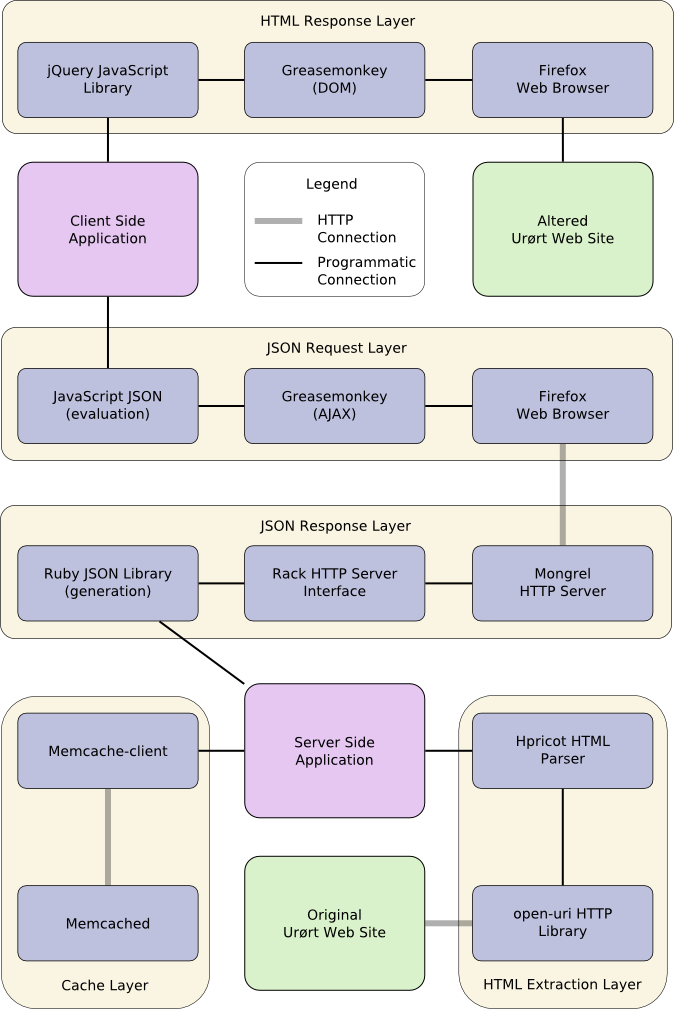
\includegraphics[width=0.9\wholewidth]{fig_prototype_architecture}
    \caption[Prototype Architecture]{
      High level view of the overall prototype architecture.
    }
    \label{figure:fig.prototype.architecture}
  \end{whole}
\end{figure}


\section{Development Tools}

As with the implementation platforms, languages, and third party libraries
our first criterion for selecting development tools is freedom.

\subsection{Version Control}

We've found it indispensable to use \term{version control} when writing code
and even used it when authoring this thesis. We'll not spend time to discuss
the merits of version control since we feel it's benefits are major and
using one induces almost zero overhead in your working process. Sometimes we
feel that the use of version control can guide you when conducting complex
tasks.

There are however several different forms of version control system one can
use. One of the most used version control implementations the last years
in open source circles was
\project{Subversion}%
\sidenote[-8\onelineskip]{
  Available at \url{http://subversion.tigris.org}.
}\dash{}a \term{centralized version control system} meaning that one central
server holds the version controlled code repository and it's history.%
\sidenote[-7\onelineskip]{
  Developers on the client side have working copies and need to contact the
  centralized server to get a hold of historical data and create new history.
}
Recently \term{decentralized version control systems} have become more popular
amongst developers. A decentralized model means that every developer can have
their own repository consisting of all history.%
\sidenote[-5\onelineskip]{
  You can for instance be without internet connectivity and still commit
  changes, revert to previous versions, and handle all other tasks your
  version control system supports.
}
Code is then shared either in a push or pull fashion between such individual
repositories. This enables a much better model for collaboration.
We favor this last model of version control and so have projects
like \project{Linux}, \project{X}, \project{Mozilla},
and \project{OpenSolaris}.%
\sidenote[-3\onelineskip]{
  \citeauthor{torvalds07}, author of the Linux kernel,
  have described Subversion and centralized version control
  as fundamentally flawed since it's supposed to be a
  \q{\abbr{CVS} done right}. Since he feels \abbr{CVS} is flawed Subversion
  is therefore inherently flawed \citeyearpar{torvalds07}.
}

Based on criteria of performance and current adoption there are in our view
only two interesting decentralized version control systems:
\project{Git}%
\sidenote{
  Available at \url{http://git.or.cz}.
}
and \project{Mercurial}%
\sidenote{
  Available at \url{http://www.selenic.com/mercurial}.
}. Both are unique in that they don't track meta-data, they just track
content and meta-data are thereby inferred from the content.
At a very high level view Mercurial have a better user interface and Git
supports some advanced features the former don't have. We opted to used
Mercurial for this development project since we've substantial experience in
using it and did not need any of Git's advanced features.

\subsection{Editor}

A developer's main tool for authoring software is his editor. Sometimes the
language of implementation warrants a specialized editor with aids for
handling cumbersome tasks specific to that language. Such an editor is often
called an \abbr{IDE}%
\sidenote[-7\onelineskip]{
  A good example of an \abbr{IDE} (integrated development environment
  for short) is \project{Eclipse} (available at \url{http://eclipse.org}).
  It was first used for Java development but since extended with
  plugins for handling other programming languages and families.
}
and are used most often for languages like Java and C\#.
\citet{murphy06} found that developers mostly use an \abbr{IDE} for navigating
large collections of source code, refactoring code, debugging code, and
interacting with revision control systems in addition to normal editor usage.
Development environments found in Lisp%
\sidenote[-4\onelineskip]{
  \prequote[p.~69]{sandewall78}{%
    describes the nature and benefits of the Lisp environment as}{%
      The `residential' design of programing systems, whereby all facilities
      for the user are integrated into one system with which the user
      communicates during the entire interactive session, offers great
      possibilities for user convenience}
}
and Smalltalk%
\sidenote{
  Similar to Lisp's programming environment
  \postquote[p.viii]{goldberg83}{%
    Smalltalk is designed so that every component in the system that is
    accessible to the user can be presented in a meaningful way for
    observation and manipulation}

}
are surpassing \abbr{IDE} types in integration and interactiveness even though
they preceded them.

The programming languages we previously settled on, JavaScript and Ruby,
are very expressive and dynamic in their nature in addition to being
interpreted instead of compiled. Our experience is that \abbr{IDE} usage for
such languages stands more in the way than aid you as a programmer during
your problem solving process.
\citet{bray07} conducted a rather unscientific survey of 1000 Ruby
programmers. Despite of the surveys shortcomings it showed that
the majority of Ruby programmers used non-\abbr{IDE} editors for their
development.

The interactive experience provided by Lisp and Smalltalk implementations are
sadly missing%
\sidenote{
  Ruby has an interactive interpreter similar to those found in Lisp and
  Smalltalk environments called \executable{irb}. It's not integrated into an
  overall programming environment and therefore is mostly used for testing out
  small ideas.
}
from JavaScript and Ruby implementations. This means that we're left with
finding a good editor which enables us to focus on writing code as efficiently
and safely as possible. Editor selection is highly a matter of preference and
finding one that matches your work process. Powerful editors have a
reputation of being quite hard to learn. But if you get over the steep
learning curve the benefits the editor gives you are worth it.

\begin{fullquote}{orenstein08}{%
  have experienced how much effort programmers can
  invest in something seemingly trivial as an editor}
    If the thought of switching editors doesn't fill you with quite a bit of
    dread, what you're using now is almost certainly under powered, and you
    definitely haven't customized it enough.
\end{fullquote}

    \chapter{Discussion}
\label{chapter:discussion}

This chapter will include a synthesis based on the analysis of our collected
data. The larger lines of our findings will be presented and we'll try to
represent a new and refreshed terminology for the field of social navigation
by the means of a taxonomy including patterns of navigational use.

\section{Social Navigation on the Social Web}

\subsection{No Explicit Design for Social Navigation}

It does not seem like the designers of social web pages design for social
navigation explicitly. There seem to be a trend for designing for social
interaction. An implicit by-product of such an approach seems to be
the creation of several forms of social navigation constructs.
We base this observation our studies of two large social web sites in
\chapterref{analysis} in addition to cursory observation on other social web
sites.

\subsection{Social Navigation Advice is Given by Peers}

An overlying theme of the forms of social navigation we found in the wild were
that it was created by equal peers. The construct for enabling the social
navigation are created by the web site creators. But the data that
enables navigational choices of a social nature are created by other users
like you\dash{}by the community.

Whether indirect or direct, explicit or implicit, navigational advice have to
be given by peers to be considered social navigation. In other words
navigational advice have to be given by individuals on the same horizontal
level as yourself. This means that navigational advice given by web editors
and web designers\dash{}people vertically superior to yourself\dash{}can not
be true social navigation.

%%
%% elaborate
%%


\section{Transparent Prototyping with Greasemonkey}

\subsection{For Developers}

During our development of a prototype application with Greasemonkey for
enhancing an established web page we got a feel for its pros and cons from a
development perspective.

\subsubsection{Requires No Access to the Established Implementation}

\subsubsection{Requires Little Knowledge of the Established Implementation}

\subsubsection{Requires More Work than Altering the Established Implementation}

\subsubsection{Fragile when the Established Implementation is Changed}

\subsubsection{Less Performant than the Established Implementation}

\subsection{For Users}

When we conducted a study of our prototype application with real world users
we got valuable feedback on how well such a system works for the average user.


\subsubsection{Limited in Browser Selection}

\subsubsection{Difficulties with Installing Greasemonkey}

\subsubsection{Difficulties with Installing User-Scripts}

    \chapter{Conclusion}
\label{chapter:conclusion}

The results of the research which we have provided in this thesis can be
categorized into three venues:

\begin{enum}
  \item We have given a structured overview of the field of social navigation
    as seen both in academic literature and in some noticeable social web
    sites.
  \item We have provided details of how one can implement unobtrusive
    prototypes in established spaces and the feasibility of such a technical
    approach.
  \item We have contributed knowledge of how activity streams functions as
    a social navigation technique on the \urort{} web site.
\end{enum}

Based on these three venues we'll provide the most important lessons to take
away from our research before we discuss possible future work in these fields.

\section{Lessons Learnt}

We believe there are both some theoretical and practical lessons to take away
from our research

\subsection{Social navigation}

As viewed in academic literature social navigation can mean different things.
We proposed a new definition of social navigation based on our belief in the
importance of peers in a social navigation system.%
\sidenote{
  The definition can be found in
  \sectionref{flickr.facebook.discussion.peers}.
}
This means that the information given from other people which guide navigation
have to come from peers within the system where navigation are conducted to be
considered social navigation.

Information given by the creators or 
editors of a web site are therefore not social navigation when used for
navigational purposes.
The creators can however implement structures in their web pages where users
of the system can impose information which can be used for social navigation.
One example of this divide can be found in recommender systems. Content based
recommendations is not social navigation since the information used
in the navigational process are given by the editors of the web page.
Recommendations given by collaborative filtering is on the other hand social
navigation since the navigational information is given by peers in the system.

\subsection{Unobtrusive prototyping}

Creating unobtrusive prototypes with Greasemonkey have its advantages and
disadvantages when used in real world experiments.

Greasemonkey is best fitted for situations where you don't have access to the
established web site one are prototyping on. If one have access to the inner
workings of a web site, it would probably be more efficient and easier to
implement the prototype within the established implementation. Another benefit
of modifying the web site implementation itself is the elimination of the
Greasemonkey and user-script installation process in addition to wider browser
support.

We found the major disadvantage of using Greasemonkey in a real world
experimental setting to be this complicated installation process and limited
browser support. We contribute this as the major factors for the high
non-accomplish rates we witnessed. Having conducted experiments in a
laboratory setting where users used pre-configured machines would have
mediated this problem.

\subsection{Activity streams}

Based on our experiment with activity streams on \urort{} we have provided
inconclusive findings of the success of such a social navigation technique.
We take our results as indications of the usefulness of activity streams.
Further research is needed to abandon the idea or recommend its usage.
Since we did not find any noticeable negative results towards activity streams
we can recommend implementations or prototypes of this feature in web sites
with similar dynamics as \urort{}.

\section{Future Work}

Our new definition of social navigation in light of the essentialness of peers
were based on cursory observations and more detailed analysis of two social
web sites. We regard our findings of how social navigation is used in social
web sites as early work in this area which needs to be expanded on. More
widespread collection and analysis of social navigation in modern web sites is
needed to see if our observations holds true.

We've described social navigation as a disparate field. We hope our work
some extent can remedy this problem. One venue for further work to make social
navigation a better understood term would be to create a taxonomy of social
navigation types. A set of design patterns for when, where, how, and why these
various types of social navigation should be used could accompanying such a
taxonomy.

% If we had time we would have conducted a laboratory study as well. This way
% we would not have problems with the technological seeding we've seen
% since only the most technical apt were able to complete the entire study.

% We would also have tested the prototypes over a longer time frame. Favorite
% usage numbers gave us inconclusive results. With a longer usage period there
% could be possible changes in how important favorites are.


    \begin{appendices}
      \chapter{Content Inventory}

When gathering data in the inventory phase of content analysis the root
document, the main portal to the site under investigation, was entered and
identified in an inventory table with an identifier of \emph{0}. From this
page all relevant navigational links were followed in a logical order (from
top to bottom and left to right on each page). Each new page entered by
following such links was noted down in the inventory table and given an
identifier based on it's hierarchical nature of the navigation system.

The result of this exercise were a table identifying a website's various pages
and the relationships amongst them. To better understand these relationships
content maps based on the raw data from the inventory phase were created
(Appendix~\ref{appendix:content.mapping},
p.~\pageref{appendix:content.mapping}).

\label{appendix:content.inventory}

\section{Flickr}

The following content inventory detailed in
Table~\ref{table:flickr.content.inventory}
(p.~\pageref{table:flickr.content.inventory})
represents the state of the Flickr service as of the 20th of September 2007.
Details could very well have changed since then as
services like these are known to have a rapid development cycle
where changes often are imposed on the user base at quite
a frequent rate.

When collecting data one notices that there is an enormous amount of pages
sharing a common structure only differing in a single or a few variables.
Examples include the user in question for a profile page, the tag for a
listing of photos annotated with such a tag, the date for time based history
listings and so on. I therefore introduced several such variables prefixed
with a dollar sign:
\emph{\$}\footnote{Inspired from variable usage inUNIX shell scripting}.
A complete listing of such variables and their meaning can be found in
Table~\ref{table:flickr.variable.list}
(p.~\pageref{table:flickr.variable.list})

\begin{table}
  \begin{center}
    \begin{small}

      \caption{Variable Listing for Flickr}
      \label{table:flickr.variable.list}

      \begin{tabular}{lp{8cm}}

        \toprule
        Variable & Description \\
        \midrule

        \var{user} &
        Unique nick-name for a user \\

        \var{photo-id} &
        Unique numerical identifier for a photo \\

        \var{photo-title} &
        Textual title of a photo \\

        \var{set-id} &
        Unique numerical identifier for a set (of photos) \\

        \var{set-title} &
        Textual title of a set (of photos) \\

        \var{tag} &
        Unique name for a tag \\

        \var{group} &
        Unique textual name for a group \\

        \var{camera-make} &
        Manufacturer of digital cameras \\

        \var{camera-model} &
        Model number of a particular digital camera \\

        \var{date} &
        A given date (year, optional month, and optional day) \\

        \var{topic-id} &
        Unique numerical identifier for a discussion topic \\

        \var{topic-title} &
        Textual title of a discussion topic \\

        \var{member-count} &
        Variable number of members of a group \\

        \bottomrule

      \end{tabular}
    \end{small}
  \end{center}
\end{table}

% describe the table columns

% Include this after the data has been cleaned up (use best of h1/title).
%
% Most pages have both a title displayed in the browsers title-bar (using a
% HTML title anchor inside the head anchor) and a in page-heading (usually inside
% a HTML h1 anchor). During the content inventory I took not of the most
% descriptive of these two in the following ``Page Title'' columns. There were
% occasions where one of these were lacking in properly describing the pages
% content. Since the aim of this content inventory is to get an informed picture
% of the navigational structures I simply selected the most fitting title.
% I opted to ignore noting down such inconsistencies as one probably would to
% when using content inventory as a tool for improving site architecture.


\setlength\LTleft{0pt plus 1fill minus 1fill}
  \let\LTright\LTleft

% Long multi-page table
\begin{landscape}
  \begin{small}
    \label{table:flickr.content.inventory.1}
    \begin{longtable}{rp{3cm}p{3cm}p{3cm}}
      \caption{Content Inventory of Flickr} \\

  % First page header
  \toprule
  Id & Page Title & Link Name & Link Location \\
  \midrule
  \endfirsthead

  % Remaining pages header
  \caption[]{(continued)}\\
  \toprule
  Id & Page Title & Link Name & Link Location \\
  \midrule
  \endhead

  % Footer except for last page
  \midrule
  \multicolumn{4}{l}{{Continued on Next Page\ldots}} \\
  \endfoot

  % Last page footer
  \bottomrule
  \endlastfoot

  % Data

0 &
Welcome to Flickr &
&
\\
% /

1 &
Photos from \var{user} &
You &
Global navigation \\
% /photos/\var{user}

  1.1 &
  \var{photo-title} &
  Photo thumbnail &
  Content area \\
  % /photos/\var{user}/\var{photo-id}

    1.1.1 &
    Photos from \var{user} &
    \var{user} &
    Content (comments list) \\
    % /photos/\var{user}

    1.1.2 &
    \var{set-title} - a photoset on Flickr &
    \var{set-title} (Set) &
    Right sidebar \\
    % /photos/\var{user}/sets/\var{set-id}

    1.1.3 &
    \var{group} Pool &
    \var{group} (Pool) &
    Right sidebar \\
    % /groups/\var{group}/pool

    1.1.4 &
    \var{user} photos tagged with \var{tag} &
    \var{tag} &
    Right sidebar (tag list) \\
    % /photos/\var{user}/tags/\var{tag}

      1.1.4.1 &
      Photos tagged with \var{tag} &
      public photos tagged with \var{tag} &
      Left sidebar \\
      % /photos/tags/\var{tag}

    1.1.5 &
    Explore your geotagged photos on a Map &
    (map) -> View \var{user} map &
    Right sidebar (details list) \\
    % /photos/\var{user}/\var{photo-id}/map/?view=users

    1.1.6 &
    Explore everyone's geotagged photos on a Map &
    (map) -> see more photos here &
    Right sidebar (details list) \\
    % /photos/\var{user}/\var{photo-id}/map/?view=everyone

    1.1.7 &
    Camera Finder: \var{camera-model} &
    \var{camera-model} &
    Right sidebar (detail list) \\
    % /cameras/\var{camera-make}/\var{camera-model}

    1.1.8 &
    Archive of your photos taken on \var{date} &
    \var{camera-model} &
    Right sidebar (detail list) \\
    % /photos/\var{user}/archives/date-taken/\var{date}

  1.2 &
  \var{set-title} - a photoset on Flickr &
  \var{set-title} &
  Left sidebar \\
  % /photos/\var{user}/sets/\var{set-id}

  1.3 &
  \var{user} sets on Flickr &
  Sets &
  Local navigation \\
  % /photos/\var{user}/sets

    1.3.1 &
    \var{set-title} - a photoset on Flickr &
    \var{set-title} &
    Content area \\
    % /photos/\var{user}/sets/\var{set-id}

      1.1.1.1 &
      \var{photo-title} &
      Photo thumbnail &
      Content area \\
      % /photos/\var{user}/\var{photo-id}/in/set-\var{set-id}

  1.4 &
  \var{user} tags &
  Tags &
  Local navigation \\
  % /photos/\var{user}/tags

    1.4.1 &
    \var{user} photos tagged with \var{tag} &
    \var{tag} &
    Content (tag cloud) \\
    % /photos/\var{user}/tags/\var{tag}

      1.4.1.1 &
      Photos tagged with \var{tag} &
      public photos tagged with \var{tag} &
      Left sidebar \\
      % /photos/tags/\var{tag}

      1.4.1.2 &
      \var{photo-title} &
      Photo thumbnail &
      Content area \\
      % /photos/\var{user}/\var{photo-id}


  1.5 &
  Explore your geotagged photos on a Map &
  Map &
  Local navigation \\
  % /photos/\var{user}/map

    1.5.1 &
    \$photo-name &
    Photo count icon &
    Map \\
    % /photos/\var{user}/map

      1.5.1.1 &
      \var{user} photos tagged with \var{tag} &
      \var{tag} &
      In-line dialog \\
      % /photos/\var{user}/tags/\var{tag}

      1.5.1.2 &
      \var{photo-title} &
      View photo page &
      In-line dialog \\
      % /photos/\var{user}/\var{photo-id}

  1.6 &
  Archive of all your photos on Flickr &
  Archives &
  Local navigation \\
  % /photos/\var{user}/archives

    1.6.1 &
    Archive of your photos taken on \var{date} &
    \var{date} &
    Content area (Taken on) \\
    % /photos/\var{user}/archives/date-taken/\var{date}

      1.6.1.1 &
      \var{photo-title} &
      Photo thumbnail &
      Content area \\
      % /photos/\var{user}/\var{photo-id}

    1.6.2 &
    Archive of your photos posted on \var{date} &
    \var{date} &
    Content area (Posted on) \\
    % /photos/\var{user}/archives/date-posted/\var{date}

      1.6.2.1 &
      \var{photo-title} &
      Photo thumbnail &
      Content area \\
      % /photos/\var{user}/\var{photo-id}

  1.7 &
  \var{user} favorite photos on Flickr &
  Favorites &
  Local navigation \\
  % /photos/\var{user}/favorites

    1.7.1 &
    \var{photo-title} &
    Photo thumbnail &
    Content area \\
    % /photos/\var{user}/\var{photo-id}

  1.8 &
  \var{user} most popular photos, interestingness &
  Popular &
  Local navigation \\
  % /photos/\var{user}/popular-interesting

    1.8.1 &
    \var{photo-title} &
    Photo thumbnail or photo title &
    Content area \\
    % /photos/\var{user}/\var{photo-id}

    1.8.2 &
    \var{user} most popular photos, views &
    Views &
    Sub local navigation \\
    % /photos/\var{user}/popular-views

      1.8.2.1 &
      \var{photo-title} &
      Photo thumbnail or photo title &
      Content area \\
      % /photos/\var{user}/\var{photo-id}

    1.8.3 &
    \var{user} most popular photos, favorites &
    Views &
    Sub local navigation \\
    % /photos/\var{user}/popular-faves

      1.8.3.1 &
      \var{photo-title} &
      Photo thumbnail or photo title &
      Content area \\
      % /photos/\var{user}/\var{photo-id}

    1.8.2 &
    \var{user} most popular photos, comments &
    Comments &
    Sub local navigation \\
    % /photos/\var{user}/popular-comments

      1.8.2.1 &
      \var{photo-title} &
      Photo thumbnail or photo title &
      Content area \\
      % /photos/\var{user}/\var{photo-id}

  1.9 &
  \var{user} &
  Profile &
  Local navigation \\
  % /people/\var{user}

    1.9.1 &
    Photos from \var{user} &
    \var{user} &
    Content (Groups) \\
    % /photos/\var{user}

    1.9.2 &
    \var{group} &
    \var{group} &
    Content (Groups) \\
    % /groups/\var{group}

2 &
Organize your photos &
Organize &
Global navigation \\
% /photos/organize

3 &
Photos from your contacts &
Contacts &
Global navigation \\
% /photos/friends

  3.1 &
  \var{photo-title} &
  Photo thumbnail &
  Content area \\
  % /photos/\var{user}/\var{photo-id}

  3.2 &
  Photos from \var{user} &
  \var{user} &
  Content area \\
  % /photos/\var{user}

4 &
Groups &
Groups &
Global navigation \\
% /groups

  4.1 &
  \var{group} &
  \var{group} &
  Content \\
  % /groups/\var{group}

    4.1.1 &
    \var{group} discussion topics &
    Discussion &
    Local navigation \\
    % /groups/\var{group}/discuss

      4.1.1.1 &
      \var{topic-title} in \var{group} &
      \var{topic-title} &
      Content (topic list) \\
      % /groups/\var{group}/discuss/\var{topic-id}

      4.1.1.2 &
      Photos from \var{user} &
      \var{user} &
      Content (topic list) \\
      % /photos/\var{user}

    4.1.2 &
    \var{group} Pool &
    Pool &
    Local navigation \\
    % /groups/\var{group}/discuss

      4.1.2.1 &
      \var{photo-title} &
      Photo thumbnail &
      Content area \\
      % /photos/\var{user}/\var{photo-id}/in/pool-\var{group}

      4.1.2.2 &
      Photos from \var{user} &
      \var{user} &
      Content area \\
      % /photos/\var{user}

    4.1.3 &
    Explore geotagged photos from \var{group}  &
    Pool &
    Local navigation \\
    % /groups/\var{group}/pool/map?mode=group

      4.1.3.1 &
      \$photo-name &
      Photo count icon &
      Map \\
      % /groups/\var{group}/pool/map?mode=group

        4.1.3.1.1 &
        \var{user} photos tagged with \var{tag} &
        \var{tag} &
        In-line dialog \\
        % /photos/\var{user}/tags/\var{tag}

        4.1.3.1.2 &
        \var{photo-title} &
        View photo page &
        In-line dialog \\
        % /photos/\var{user}/\var{photo-id}

    4.1.3 &
    \var{group}  &
    \var{member-count} Members &
    Local navigation \\
    % /groups\_members.gne?id=\var{group}-id

      4.1.3.1 &
      Photos from \var{user} &
      \var{user} &
      Content area \\
      % /photos/\var{user}

5 &
Explore &
Explore &
Global navigation \\
% /explore

  5.1 &
  \var{photo-title} &
  Photo thumbnail or \var{photo-title} &
  Content (highlighted photo) \\
  % /photos/\var{user}/\var{photo-id}

  5.2 &
  Photos from \var{user} &
  \var{user} &
  Content (highlighted photo) \\
  % /photos/\var{user}

  5.3 &
  Explore interesting photos from the last 7 days &
  last 7 days &
  Content area \\
  % /explore/interesting/7days

    5.3.1 &
    \var{photo-title} &
    Photo thumbnail or \var{photo-title} &
    Content area \\
    % /photos/\var{user}/\var{photo-id}

    5.3.2 &
    Photos from \var{user} &
    \var{user} &
    Content area \\
    % /photos/\var{user}

  5.4 &
  Explore interesting photos from \var{date} &
  \var{date} &
  Content area \\
  % /explore/interesting/\var{date}

    5.4.1 &
    \var{photo-title} &
    Photo thumbnail or \var{photo-title} &
    Content area \\
    % /photos/\var{user}/\var{photo-id}

    5.4.2 &
    Photos from \var{user} &
    \var{user} &
    Content area \\
    % /photos/\var{user}

  5.5 &
  Explore everyones geotagged photos on a Map &
  a map of the world &
  Content area \\
  % /map

    5.5.1 &
    \$photo-name &
    Photo count icon &
    Map \\
    % /map

      5.5.1.1 &
      \var{user} photos tagged with \var{tag} &
      \var{tag} &
      In-line dialog \\
      % /photos/\var{user}/tags/\var{tag}

      5.5.1.2 &
      \var{photo-title} &
      View photo page &
      In-line dialog \\
      % /photos/\var{user}/\var{photo-id}

  5.6 &
  Popular Tags &
  popular tags &
  Content area \\
  % /photos/tags

    5.6.1 &
    Photos tagged with \var{tag} &
    \var{tag} &
    Content (tag cloud) \\
    % /photos/tags/\var{tag}

      5.6.1.1 &
      Photos tagged with \var{tag} &
      Most interesting &
      Left column \\
      % /photos/tags/\var{tag}/interesting

        5.6.1.1.1 &
        \var{photo-title} &
        Photo thumbnail &
        Content area \\
        % /photos/\var{user}/\var{photo-id}

        5.6.1.1.2 &
        Photos from \var{user} &
        \var{user} &
        Content area \\
        % /photos/\var{user}

      5.6.1.2 &
      Photos tagged with \var{tag} &
      \var{tag} clusters &
      Left column \\
      % /photos/tags/\var{tag}/clusters

        5.6.1.2.1 &
        \var{photo-title} &
        Photo thumbnail &
        Content area \\
        % /photos/\var{user}/\var{photo-id}

        5.6.1.2.2 &
        Photos from \var{user} &
        \var{user} &
        Content area \\
        % /photos/\var{user}

        5.6.1.2.3 &
        Photos tagged with \var{tag} &
        \var{tag} &
        Content (cluster list) \\
        % /photos/tags/\var{tag}/clusters

        5.6.1.2.4 &
        Photos tagged with \var{tag} &
        See more of this cluster\ldots &
        Content area \\
        % /photos/tags/\var{tag}/clusters/\var{tag}-\var{tag}-\var{tag}

          5.6.1.2.4.1 &
          \var{photo-title} &
          Photo thumbnail &
          Content area \\
          % /photos/\var{user}/\var{photo-id}

          5.6.1.2.4.2 &
          Photos from \var{user} &
          \var{user} &
          Content area \\
          % /photos/\var{user}

      5.6.1.3 &
      \var{photo-title} &
      Photo thumbnail &
      Content area \\
      % /photos/\var{user}/\var{photo-id}

      5.6.1.4 &
      Photos from \var{user} &
      \var{user} &
      Content area \\
      % /photos/\var{user}

  5.7 &
  Camera Finder &
  Camera finder &
  Content area \\
  % /cameras

    5.7.1 &
    Camera Finder: \var{camera-make} &
    \var{camera-make} &
    Content area \\
    % /cameras/\var{camera-make}

      5.7.1.1 &
      Camera Finder: \var{camera-make}: \var{camera-model} &
      \var{camera-model} &
      Content area \\
      % /cameras/\var{camera-make}/\var{camera-model}

        5.7.1.1.1 &
        \var{photo-title} &
        Photo thumbnail &
        Content area \\
        % /photos/\var{user}/\var{photo-id}

        5.6.1.1.2 &
        Photos from \var{user} &
        \var{user} &
        Content area \\
        % /photos/\var{user}

  5.8 &
  Photos from everyone &
  most recent uploads &
  Content area \\
  % /photos

      5.8.1 &
      \var{photo-title} &
      Photo thumbnail &
      Content area \\
      % /photos/\var{user}/\var{photo-id}

      5.8.2 &
      Photos from \var{user} &
      \var{user} &
      Content area \\
      % /photos/\var{user}

      5.8.3 &
      Popular Tags &
      Popular tags &
      Right sidebar \\
      % /photos/tags

      5.8.4 &
      Creative Commons &
      Creative Commons &
      Right sidebar \\
      % /creativecommons

        5.8.4.1 &
        \var{photo-title} &
        Photo thumbnail &
        Content area \\
        % /photos/\var{user}/\var{photo-id}

        5.8.4.2 &
        Photos from \var{user} &
        \var{user} &
        Content area \\
        % /photos/\var{user}

        5.8.4.3 &
        Photos with Creative Commons \$license-type &
        See more &
        Content (\$license-type) \\
        % /photos/\var{user}

          5.8.4.3.1 &
          \var{photo-title} &
          Photo thumbnail &
          Content area \\
          % /photos/\var{user}/\var{photo-id}

          5.8.4.3.2 &
          Photos from \var{user} &
          \var{user} &
          Content area \\
          % /photos/\var{user}

  5.9 &
  Photos tagged with \var{tag} &
  \var{tag} &
  Content (tag cloud) \\
  % /photos/tags/\var{tag}


  5.10 &
  Explore interesting photos from \var{date} &
  \var{date} &
  Content (A year ago) \\
  % /explore/interesting/\var{date}

    5.10.1 &
    \var{photo-title} &
    Photo thumbnail &
    Content area \\
    % /photos/\var{user}/\var{photo-id}

    5.10.2 &
    Photos from \var{user} &
    \var{user} and see more photos &
    Content area \\
    % /photos/\var{user}

    5.10.3 &
    \var{user} &
    profile &
    Content area \\
    % /people/\var{user}

    5.10.4 &
    Photos tagged with \var{tag} &
    \var{tag} &
    Content area \\
    % /photos/tags/\var{tag}/clusters

  5.11 &
  \var{photo-title} &
  Photo thumbnail or \var{photo-title} &
  Content (A year ago) \\
  % /photos/\var{user}/\var{photo-id}

  5.12 &
  Photos from \var{user} &
  \var{user} &
  Content (A year ago) \\
  % /photos/\var{user}

  5.13 &
  \var{user} &
  profile &
  Content (A year ago) \\
  % /people/\var{user}

  5.14 &
  \var{set-title} - a photoset on Flickr &
  \var{set-title} &
  Content (Sets) \\
  % /photos/\var{user}/sets/\var{set-id}

    5.14.1 &
    \var{photo-title} &
    Photo thumbnail &
    Content area \\
    % /photos/\var{user}/\var{photo-id}/in/set-\var{set-id}

  5.15 &
  Photos from \var{user} &
  \var{user} &
  Content (Sets) \\
  % /photos/\var{user}

  5.16 &
  Groups &
  loads of groups &
  Content (Groups) \\
  % /groups

  5.17 &
  \var{group} &
  \var{group} &
  Content (Groups) \\
  % /groups/\var{group}

  5.18 &
  \var{group} Pool &
  Pool &
  Local navigation \\
  % /groups/\var{group}/pool

  5.19 &
  \var{group}  &
  \var{member-count} Members &
  Local navigation \\
  % /groups\_members.gne?id=\var{group}-id

    \end{longtable}
  \end{small}
\end{landscape}

\section{Amazon}

\section{Facebook}

\section{Del.icio.us}

      \chapter{Questionnaire}
\label{appendix:questionnaire}

\section{User Profile}

Questions to determine who the respondent is and his or hers usage of
\urort{}.

\begin{items}
  \item Hvor gammel er du? [0-19, 20-29, 30-40, 40-]
  \item Hvilket kjønn er du? [mann, kvinne]
  \item Hvor ofte bruker du \urort{}?
    [daglig, ukentlig, månedlig, skjelden, aldri]
  \item I hvilken tilstand benytter du oftest \urort{}? [innlogget, anonymt]
  \item Hvor ofte bruker du tjenester på web som støtter sosiale
    nettverk (eksempelvis Facebook, Myspace, last.fm, Flickr, Underskog
    og så videre)?
    [daglig, uketlig, månedlig, skjelden, aldri]
\end{items}

\section{Favorites on \urort{}}

Questions to determine the respondent's familiarity with favorites and use of
favorites on \urort{}.

\begin{items}
  \item Er du kjent med begrepet \q{favoritter} på \urort{}? [ja, nei]
  \item Hvor mange favoritter har du på \urort{}? [0, 1-9, 10-20, 20-50, 50-]
  \item Hva slags kriterier benytter du når du velger favoritter på
    \urort{}? [musikk, kjennskap, vennskap, popularitet]
  \item Hvor ofte bruker du favoritter på \urort{}?
    [daglig, ukentlig, månedlig, skjelden, aldri]
  \item Hva bruker du favoritter til på \urort{}?
    [holde meg oppdatert, vise støtte, annet]
\end{items}

\section{Usefulness}

Questions to determine the respondent's percieved usefulness of new
functionality before and after actual usage.

\begin{items}
  \item Bruk av \siste{} vil la meg fullføre mine oppgaver på \urort{}
    raskere.
    [veldig sannsynlig, ganske sannsynlig, litt sannsynlig,
    verken sannsynlig eller usannsynlig,
    litt usannsynlig, ganske usannsynlig, veldig usannsynlig,]
  \item Bruk av \siste{} vil øke min produktivitet på \urort{}.
    [veldig sannsynlig, ganske sannsynlig, litt sannsynlig,
    verken sannsynlig eller usannsynlig,
    litt usannsynlig, ganske usannsynlig, veldig usannsynlig,]
  \item Bruk av \siste{} vil gjøre bruken av \urort{} lettere.
    [veldig sannsynlig, ganske sannsynlig, litt sannsynlig,
    verken sannsynlig eller usannsynlig,
    litt usannsynlig, ganske usannsynlig, veldig usannsynlig,]
  \item Jeg ville finne \siste{} nyttig på \urort{}.
    [veldig sannsynlig, ganske sannsynlig, litt sannsynlig,
    verken sannsynlig eller usannsynlig,
    litt usannsynlig, ganske usannsynlig, veldig usannsynlig,]
\end{items}

\section{Ease of Use}

Questions to determine the respondent's percieved ease of use for new
functionality before and after actual usage.

\begin{items}
  \item Lære å bruke \siste{} ville være lett for meg på \urort{}.
    [veldig sannsynlig, ganske sannsynlig, litt sannsynlig,
    verken sannsynlig eller usannsynlig,
    litt usannsynlig, ganske usannsynlig, veldig usannsynlig,]
  \item Min interaksjon med \siste{} ville være klar og forståelig
    på \urort{}.
    [veldig sannsynlig, ganske sannsynlig, litt sannsynlig,
    verken sannsynlig eller usannsynlig,
    litt usannsynlig, ganske usannsynlig, veldig usannsynlig,]
  \item Det ville være lett for meg å bli dyktig i bruken av \siste{}
    på \urort{}.
    [veldig sannsynlig, ganske sannsynlig, litt sannsynlig,
    verken sannsynlig eller usannsynlig,
    litt usannsynlig, ganske usannsynlig, veldig usannsynlig,]
  \item Jeg ville finne \siste{} lett å bruke på \urort{}.
    [veldig sannsynlig, ganske sannsynlig, litt sannsynlig,
    verken sannsynlig eller usannsynlig,
    litt usannsynlig, ganske usannsynlig, veldig usannsynlig,]
\end{items}


      \chapter{Source Code}

\section{Reddit Collaborative Filtering Algorithm}
\label{section:source.code.reddit}

Here is the source code of the algorithm that decides the score of a
submission. We made syntactical changes to make the code's intent clearer.

\begin{scode}{Python}{reddit.cf.algorithm}{%
  Reddit Collaborative Filtering Algorithm}{%
  The collaborative filtering algorihm used on Reddit}
\begin{lstlisting}
from datetime import datetime, timedelta
from math import log

def seconds_since_cutoff(date):
    cutoff = datetime(2005, 12, 8, 7, 46, 43)
    td = date - cutoff

    seconds = td.days * 24 * 60 * 60
    seconds += td.seconds
    seconds += float(td.microseconds) / 1000000
    return seconds

def score(up_votes, down_votes, submitted_date):
    score = up_votes - down_votes
    order = log(max(abs(score), 1), 10)
    sign = 1 if score > 0 else -1 if score < 0 else 0

    age = seconds_since_cutoff(submitted_date)

    return round(order + sign * age / 45000, 7)
\end{lstlisting}
\end{scode}


\section{JavaScript Comment Stripper}
\label{section:source.code.javascript.comment.stripper}

This small script was written to help
compare different JavaScript libraries:


\begin{scode}{Ruby}{javascript.comment.sripping}{%
  JavaScript Comment Stripping}{%
  Strips comments from JavaScript libraries}
\begin{lstlisting}
#!/usr/bin/env ruby

js_files = Dir['*.js']

ignore_pattern = /^[\s\t]?(\/\*|\*|\/\/)/

js_files.each do |file|
  File.open("#{file}.out", 'w') do |out| 
    out.puts File.readlines(file).reject do |line|
      line =~ pattern
    end
  end
end
\end{lstlisting}
\end{scode}

\section{Shell File and Directory Hierarchy}
\label{section:source.code.hierarchy}

This one-liner was used for conveying the directory and file hierarchy of our
server side software:

\begin{scode}{sh}{file.directory.hierarchy}{%
  \abbr{UNIX} File and Directory Hierarchy}{%
  File and directory hierarcy with standard \abbr{UNIX} tools}
\begin{lstlisting}
find . | sed -e 's/[^\/]*\//|--/g' -e 's/-- |/|/g'
\end{lstlisting}
\end{scode}



    \end{appendices}

  \backmatter
    \bibliographystyle{uio}
    \bibliography{bibliography}
\end{document}
